\documentclass{beamer}

\usetheme[subsectionpage=progressbar]{metropolis}

\usepackage{tikz}
\usetikzlibrary{babel}
\usetikzlibrary{arrows,shapes,positioning,shadows,trees,calc,fit}
\usetikzlibrary{overlay-beamer-styles} % 'visible on' option for nodes
\usepackage{adjustbox}


\title{Résolution de niveaux du Sokoban}
\date{\today}
\author{PoulpoGaz, darth-mole}
\institute{Candidat n° 012345}

\usepackage{graphics}
\graphicspath{{../../assets/}}
\usepackage{subcaption}

% French language support (e.g. date format)
\usepackage[french]{babel}
\usepackage[T1]{fontenc}
\usepackage{lmodern} % for missing fonts (e.g. italic in titles)

\newenvironment{customtree}{
    \begin{tikzpicture}
        [sibling distance = 10em,
        level distance = 6em,
        every node/.style = {
            shape=rectangle,
            draw,
            scale=0.85
        },
        dot/.style = {
            font = \Large
        },
        edge from parent path = {
            (\tikzparentnode) |-                          % Start from parent
            ($(\tikzparentnode)!0.5!(\tikzchildnode)$) -| % make an ortho line to mid point
            (\tikzchildnode)                              % make another ortho to the target
        }
    ]
}{
    \end{tikzpicture}%
}

\begin{document}

    \maketitle

    \section{Introduction}
        \begin{frame}{Le jeu du Sokoban}
            \begin{columns}[onlytextwidth]
                \begin{column}{0.32\textwidth}
                    \begin{figure}
                        \centering
                        \copyrightbox[b]{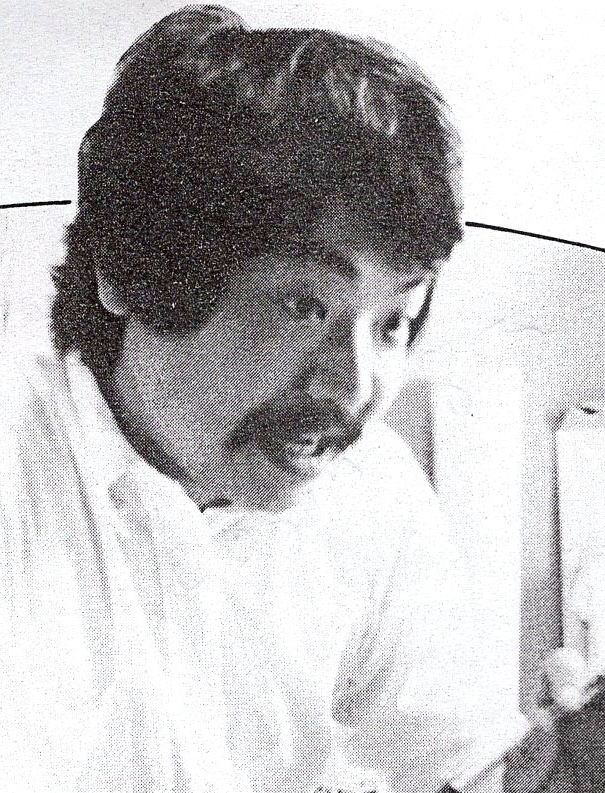
\includegraphics[width=\columnwidth]{creator.jpg}}
                                        {\url{https://shmuplations.com/wp-content/uploads/2022/03/thinkingrabbit04.jpg}}%
                        \caption*{Hiroyuki Imabayashi}
                    \end{figure}
                \end{column}
                \begin{column}{0.6\textwidth}
                    \begin{figure}
                        \centering
                        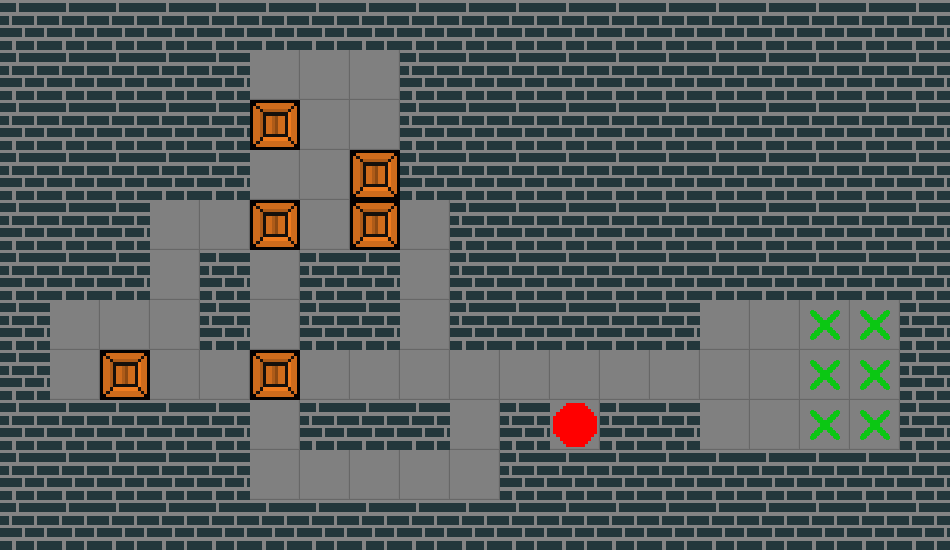
\includegraphics[width=\columnwidth]{level_example.png}
                        \caption*{\textit{XSokoban}}
                    \end{figure}
                \end{column}
            \end{columns}

            \centering
            Problème \textbf{PSPACE-complet}
        \end{frame}

        \begin{frame}{But du jeu}
            \centering
            \resizebox{\textwidth}{!}{%
                \begin{tikzpicture}
                    \node (start) {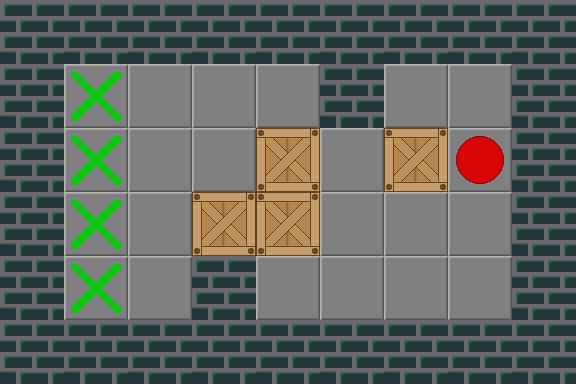
\includegraphics[width=0.5\textwidth]{rules/game_start.png}};
                    \node (end) [right=of start]{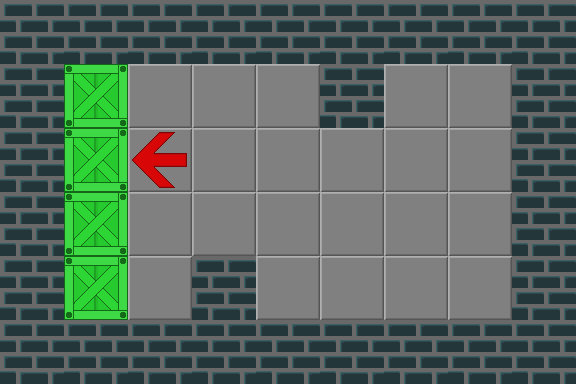
\includegraphics[width=0.5\textwidth]{rules/game_end.png}};
                    \draw[->, line width=\arrowwidth] (start.north east) to[out=60,in=130] node (label) [anchor=south, midway] {Déplacements} (end.north west);
                \end{tikzpicture}
            }
        \end{frame}

        \begin{frame}{Règles}
            \begin{columns}
                \begin{column}{0.5\textwidth}
                    \only<1-2>{
                        \begin{figure}
                            \centering
                            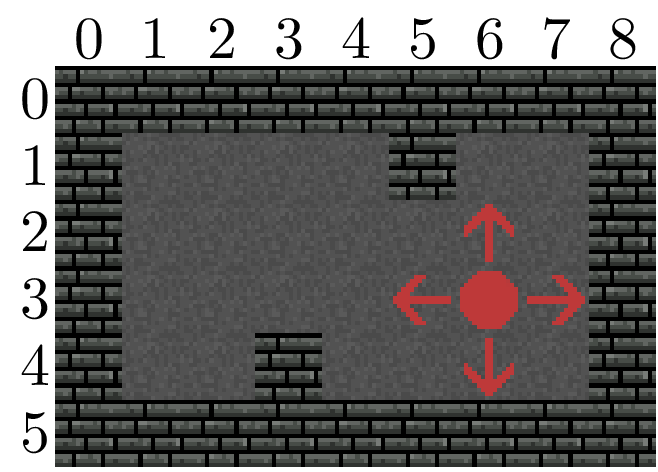
\includegraphics[width=0.9\textwidth]{rules/moves.png}
                            % \resizebox{!}{\iconwidth}{}
                            \caption*{Déplacements autorisés}
                        \end{figure}
                    }
                    \only<3>{
                        \begin{figure}
                            \centering
                            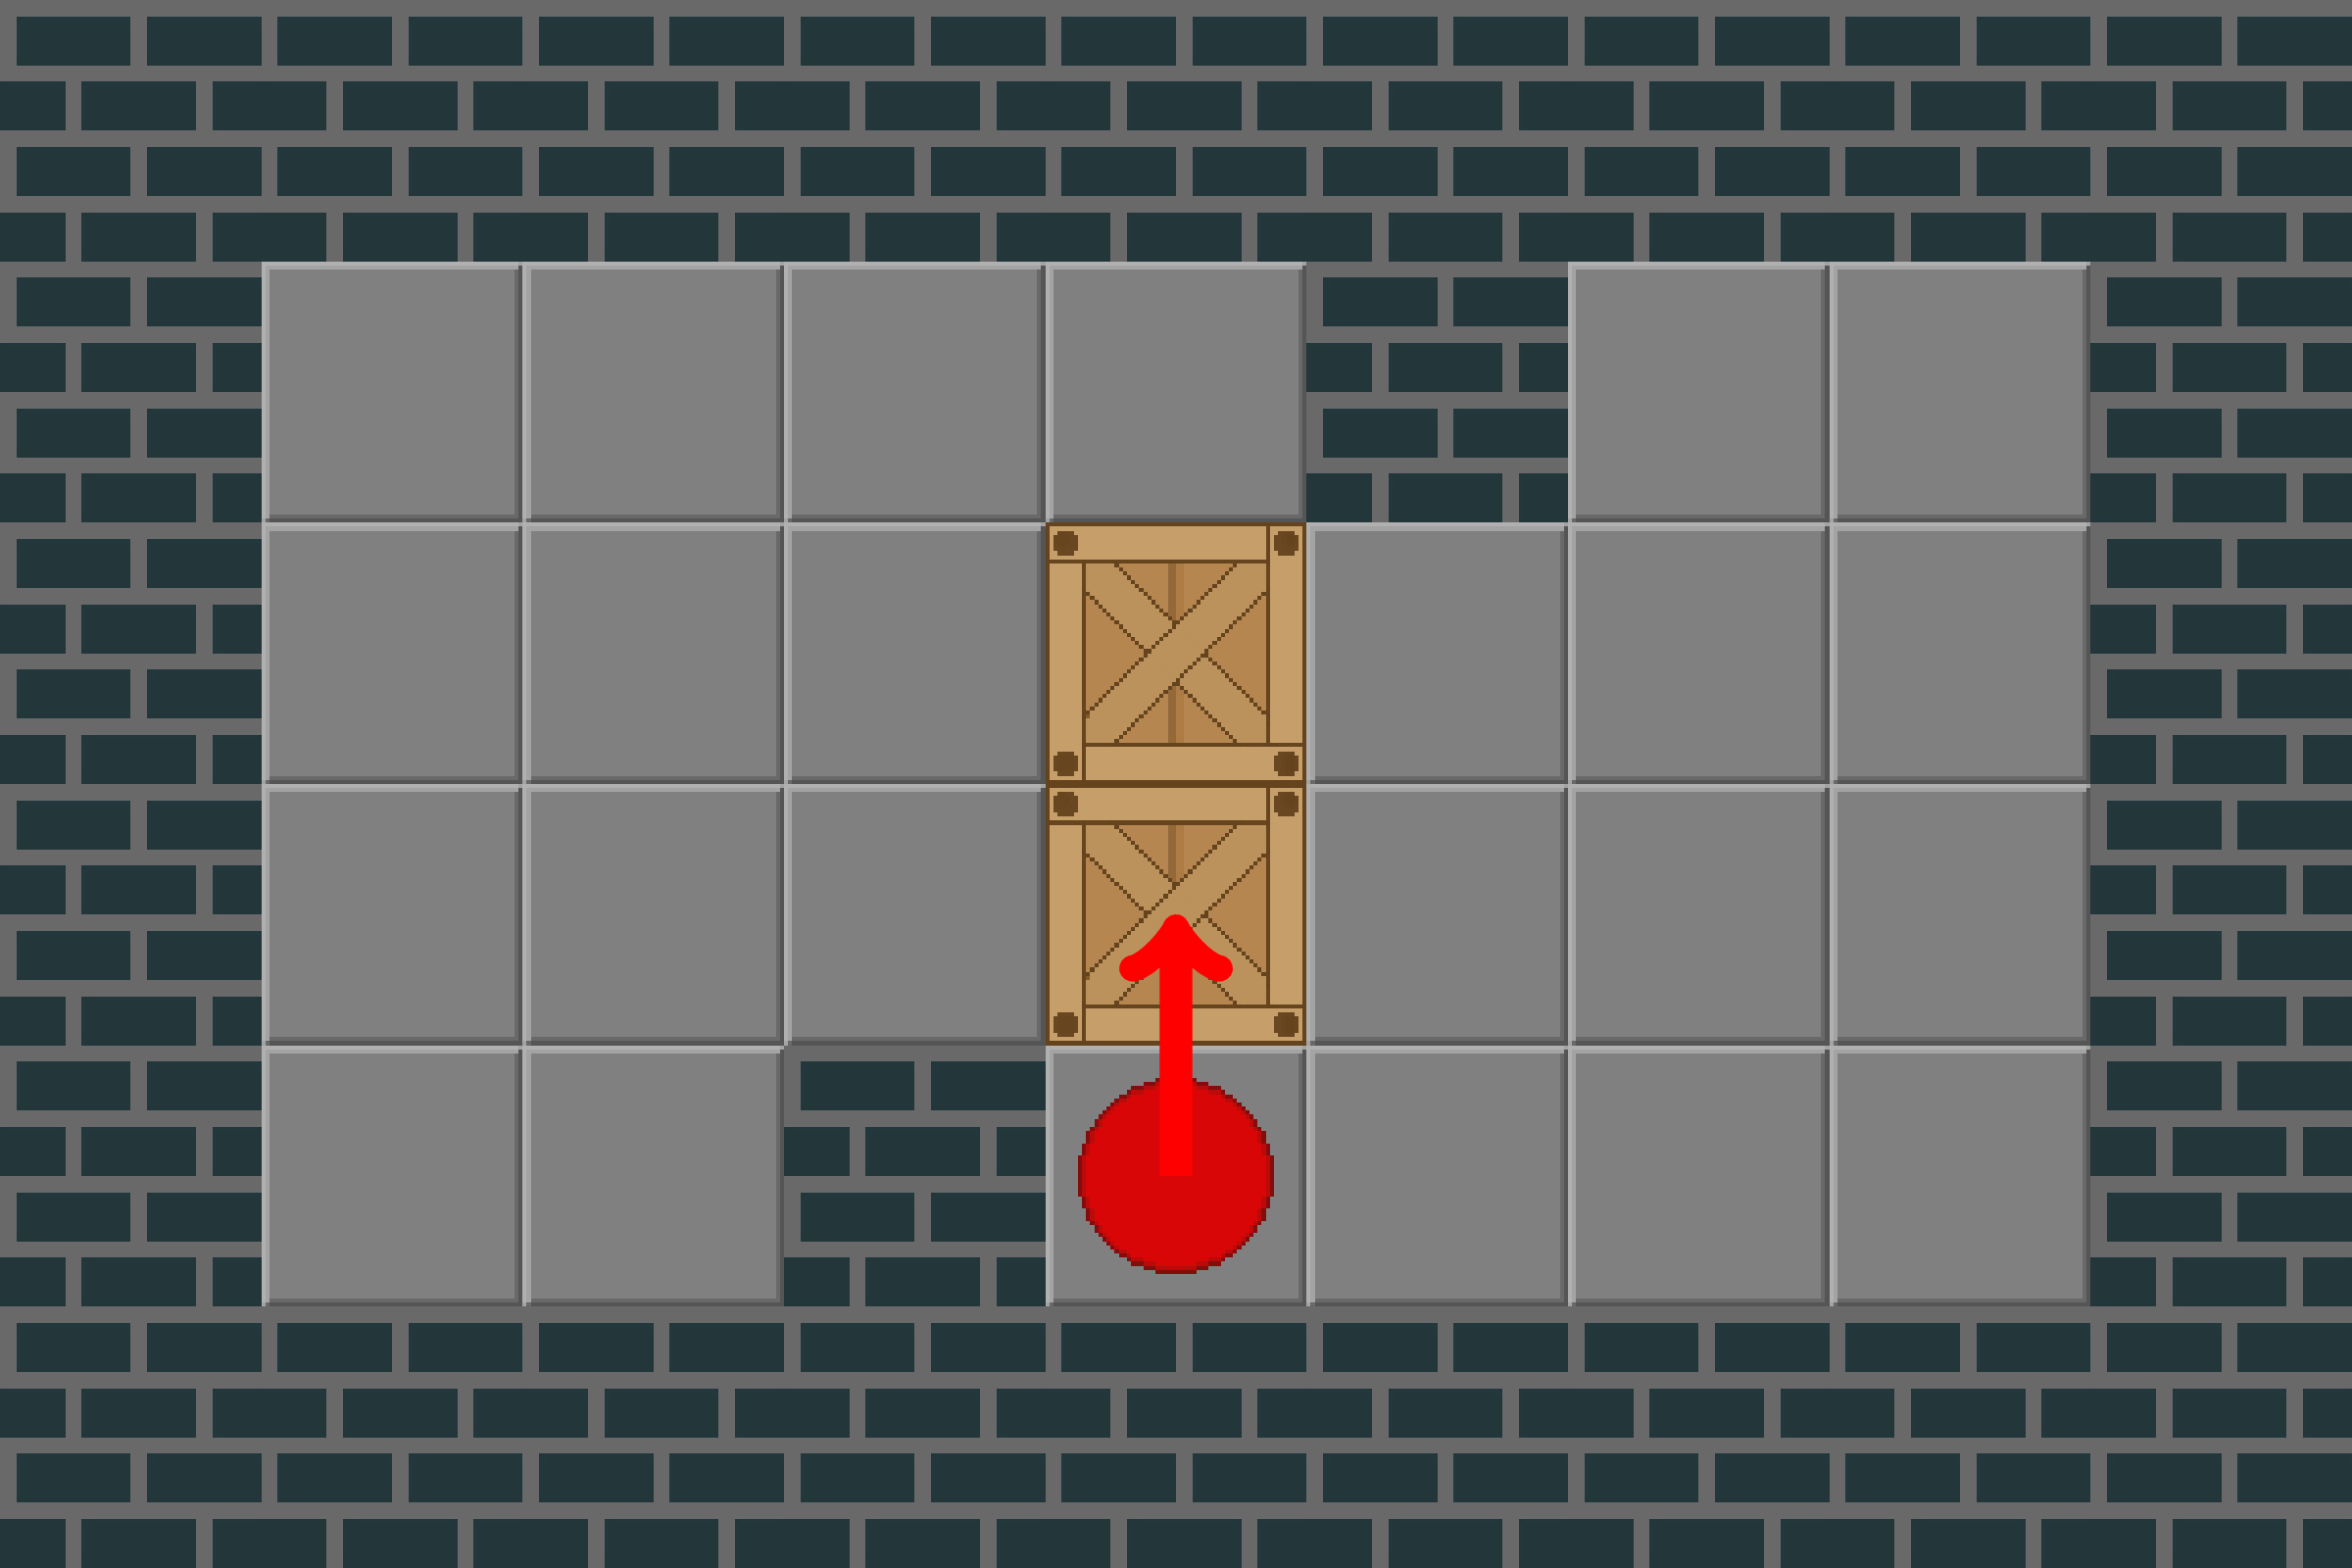
\includegraphics[width=0.9\textwidth]{rules/move_no_1.png}
                            \caption*{
\includegraphics[width=\iconwidth]{icons/no.png}}
                        \end{figure}
                    }
                \end{column}
                \begin{column}{0.5\textwidth}
                    \only<2>{
                        \begin{figure}
                            \centering
                            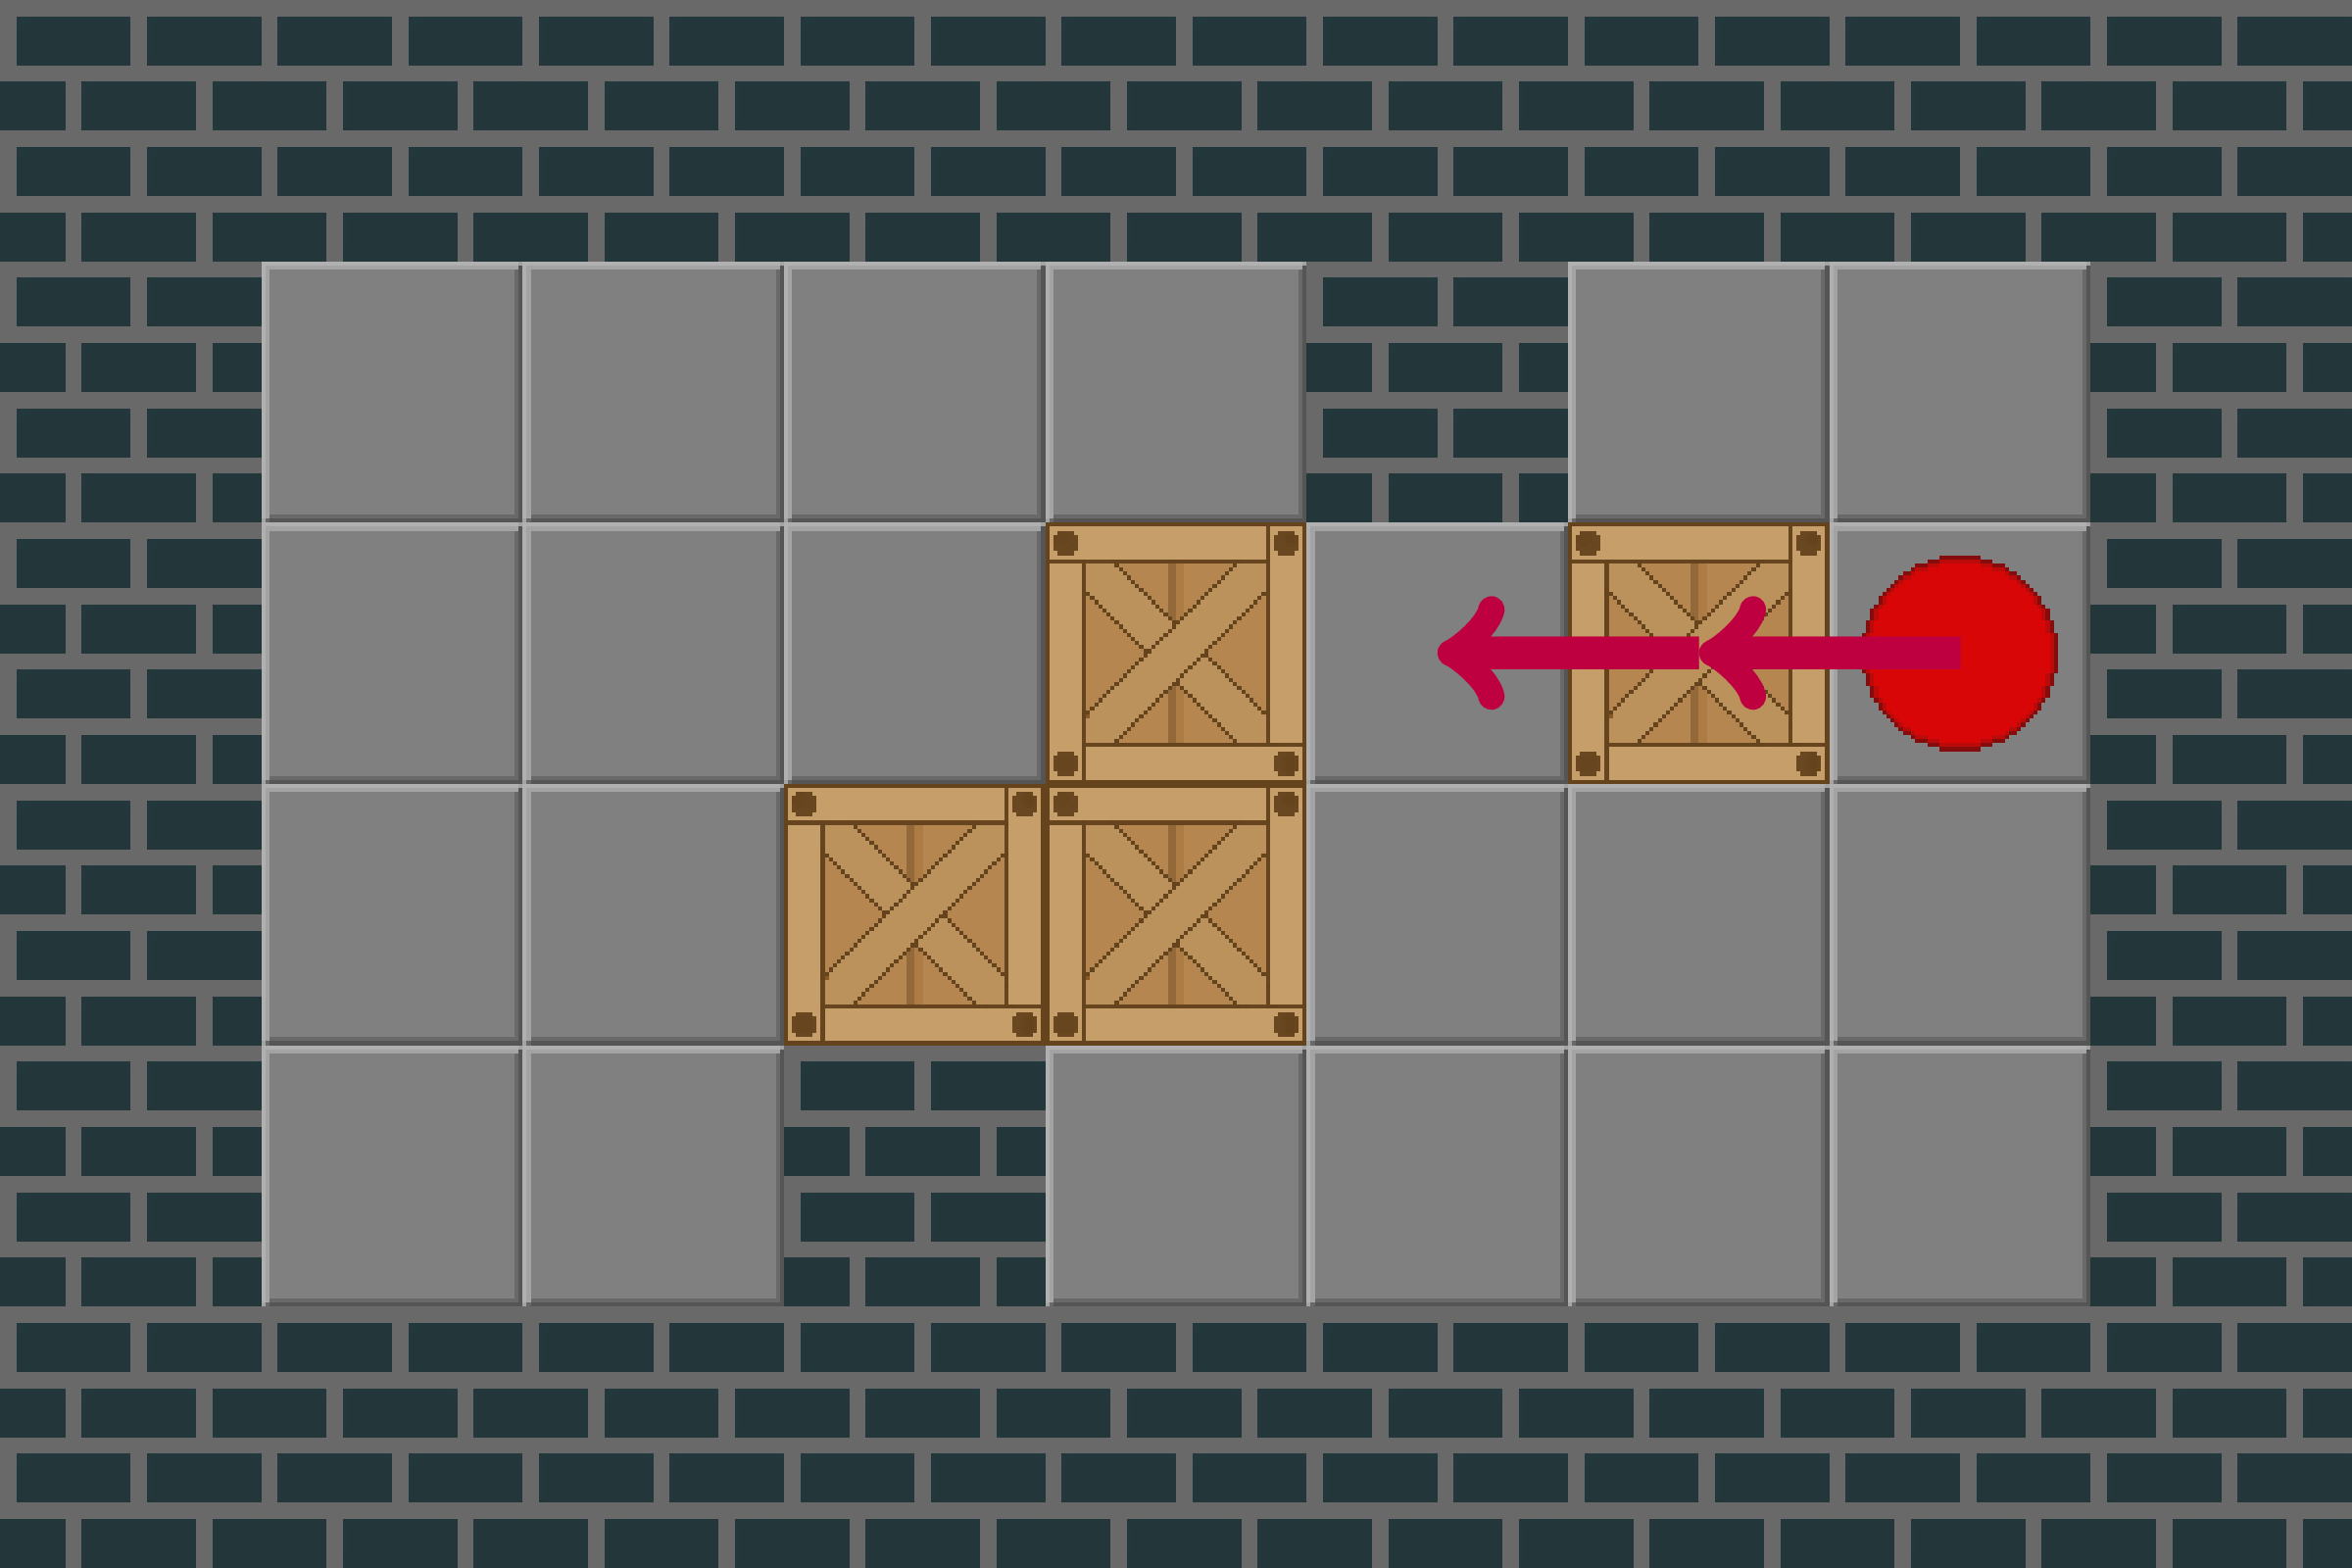
\includegraphics[width=0.9\textwidth]{rules/move_yes.png}
                            \caption*{
\includegraphics[width=\iconwidth]{icons/yes.png}}
                        \end{figure}
                    }
                    \only<3>{
                        \begin{figure}
                            \centering
                            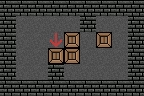
\includegraphics[width=0.9\textwidth]{rules/move_no_2.png}
                            \caption*{
\includegraphics[width=\iconwidth]{icons/no.png}}
                        \end{figure}
                    }
                \end{column}
            \end{columns}
        \end{frame}

        \begin{frame}{Tuiles}
            \centering

            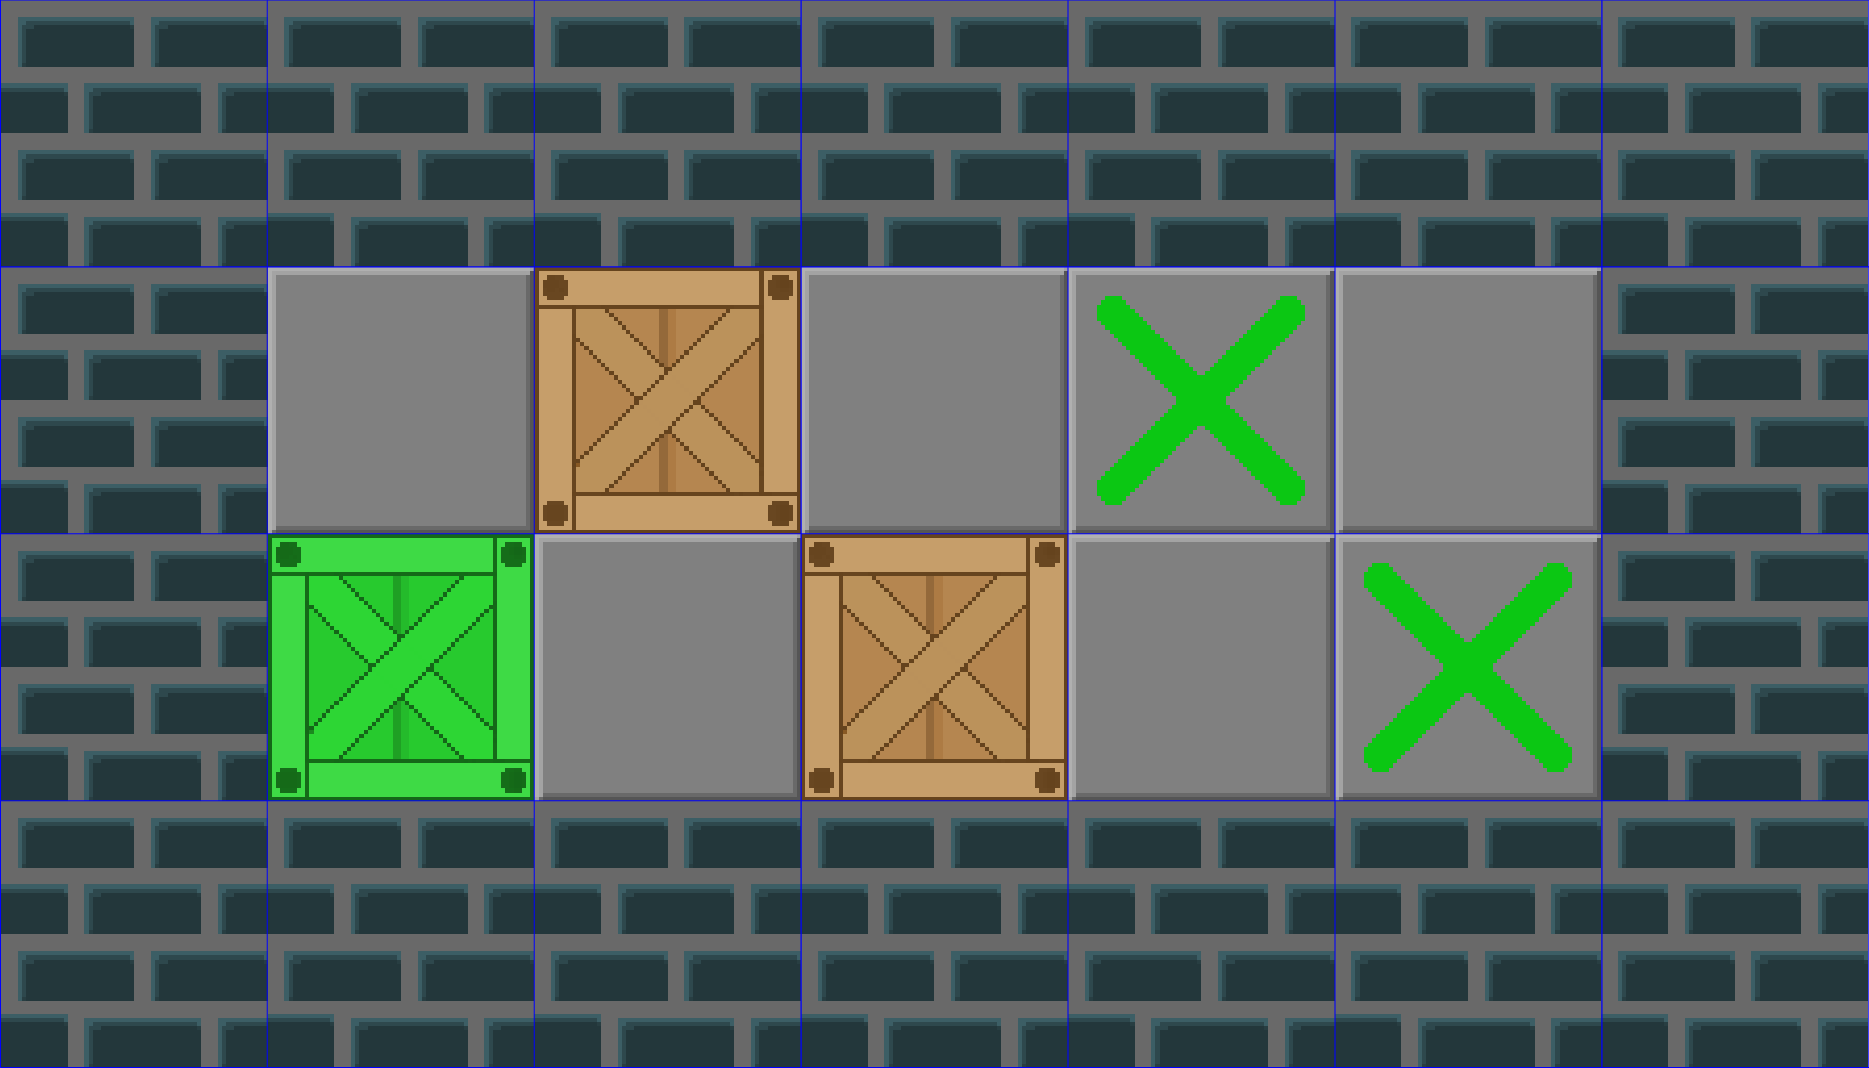
\includegraphics[width=0.5\textwidth]{tiles/tilemap.png}

            \resizebox{\textwidth}{!}{%
                \begin{tabular}{ c c c c c }
                    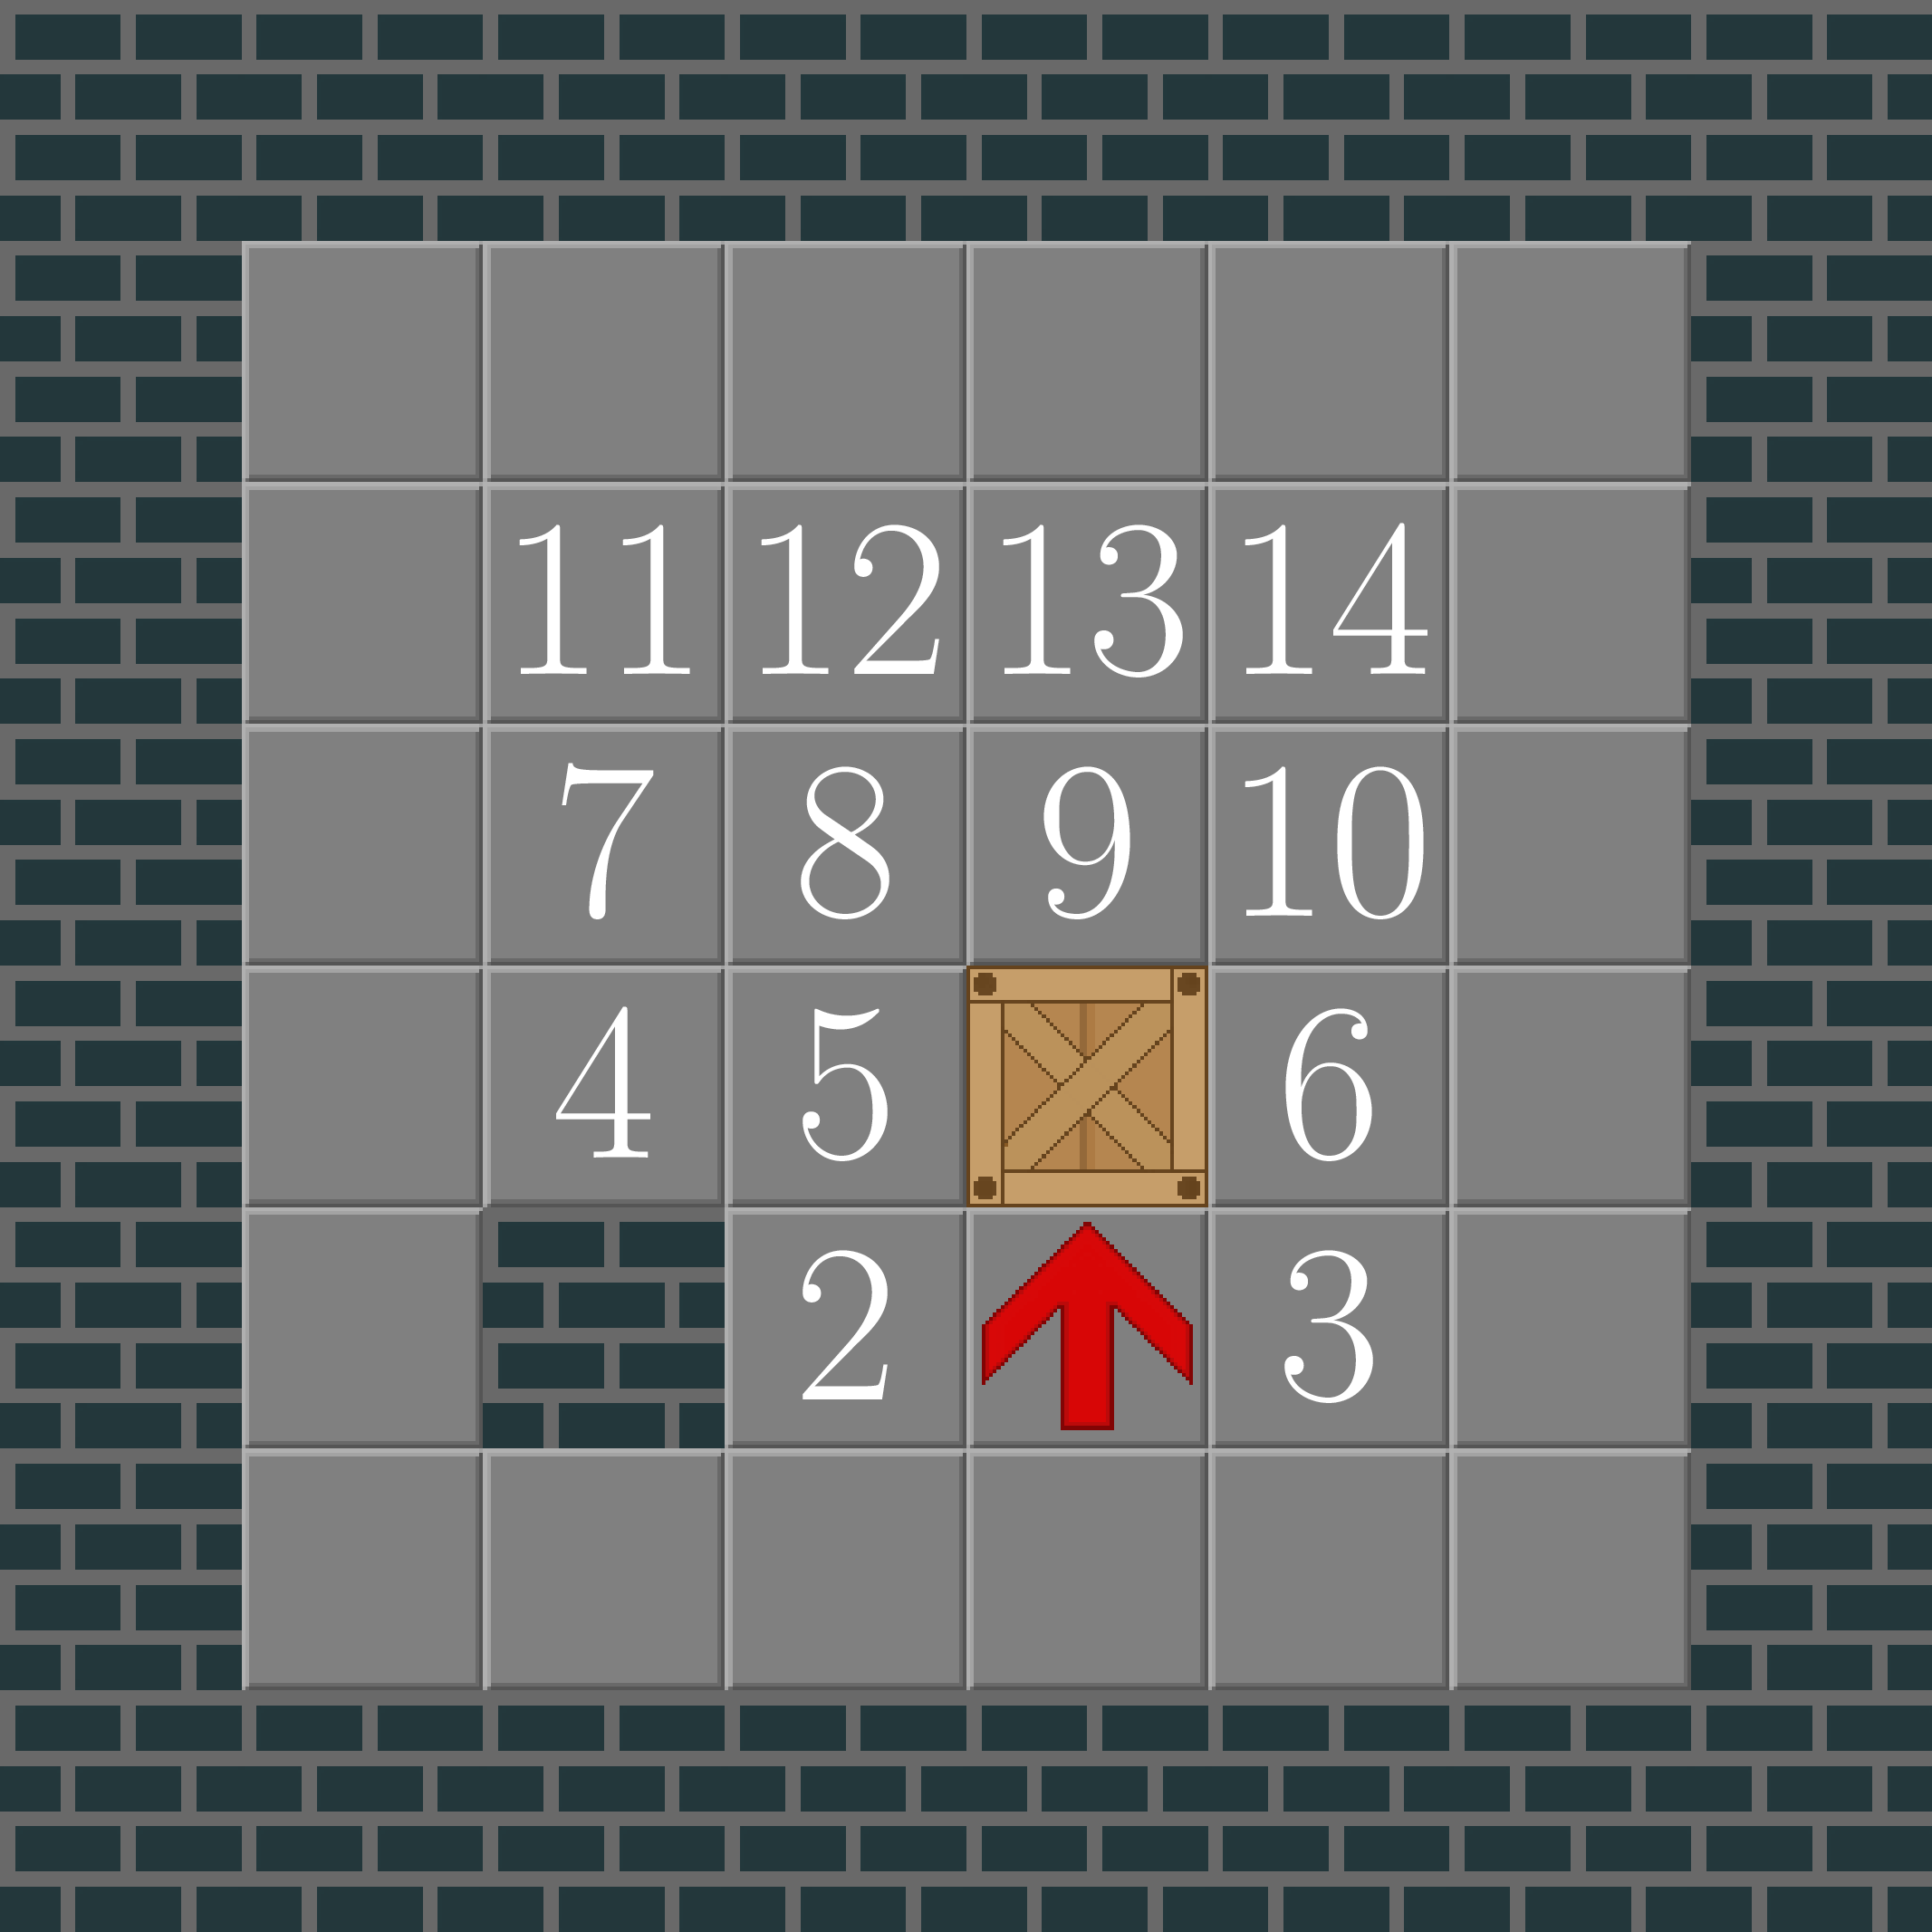
\includegraphics[width=0.2\textwidth]{tiles/wall.png} &
                    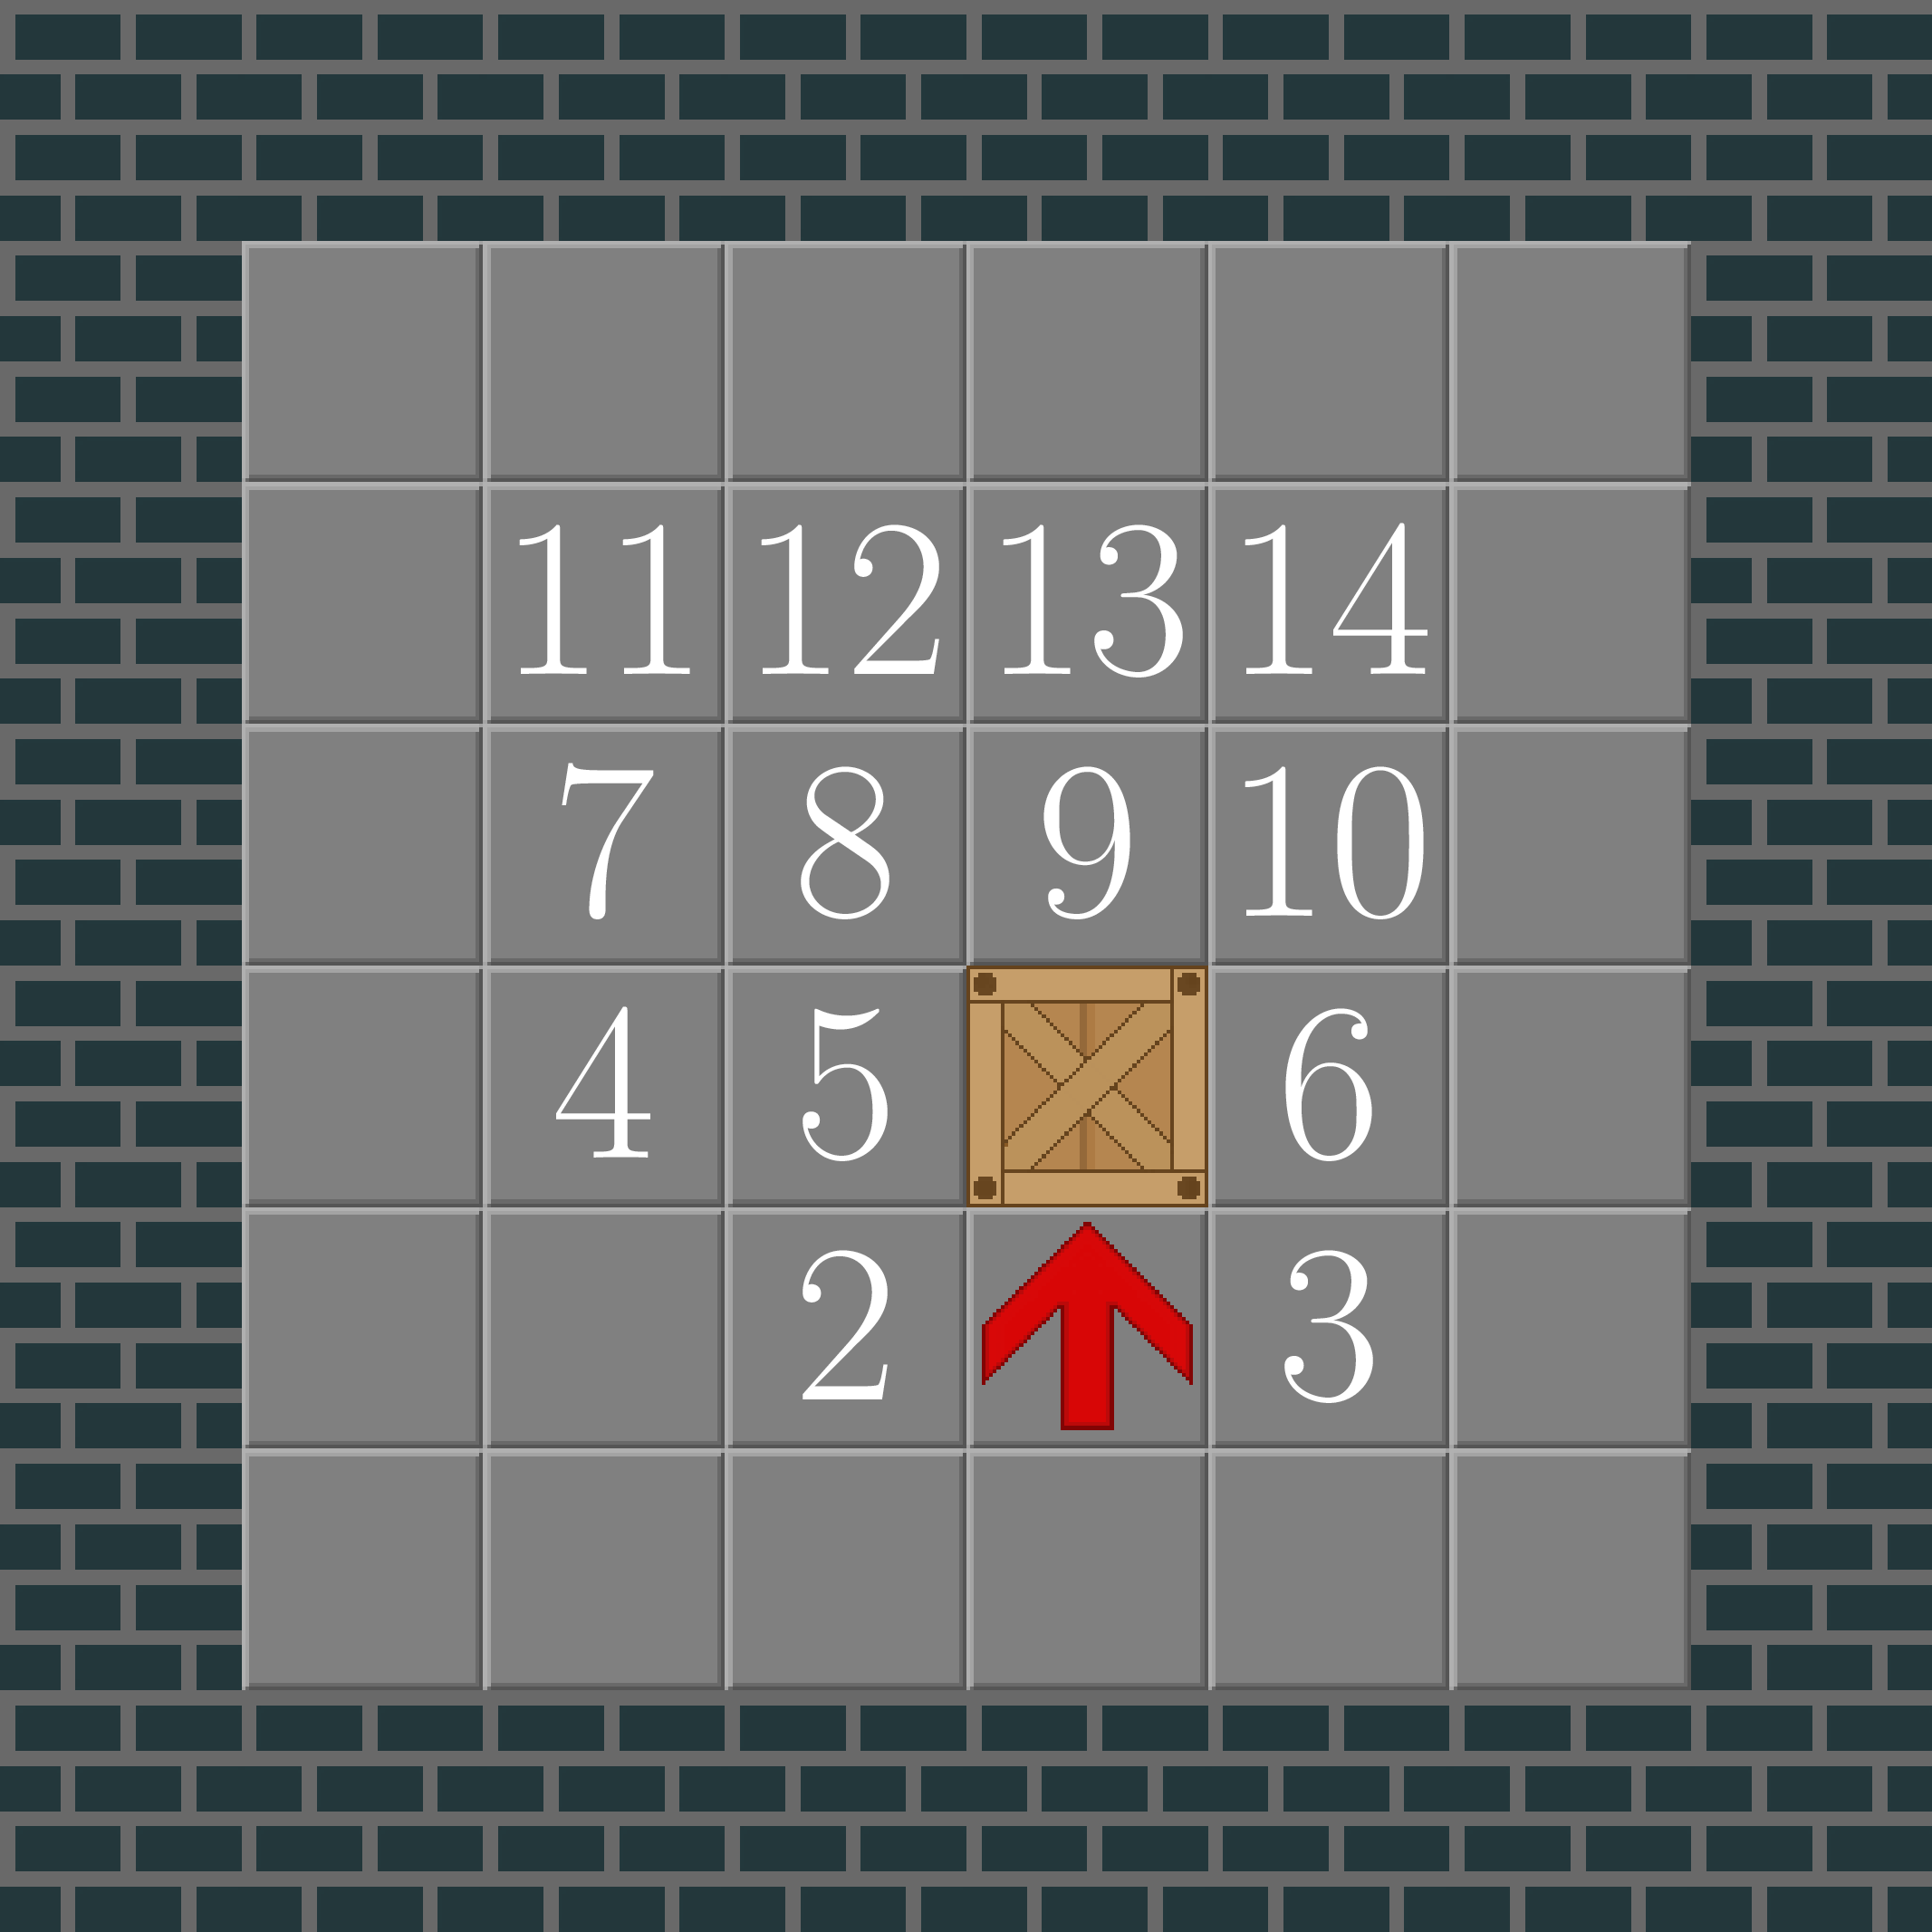
\includegraphics[width=0.2\textwidth]{tiles/floor.png} &
                    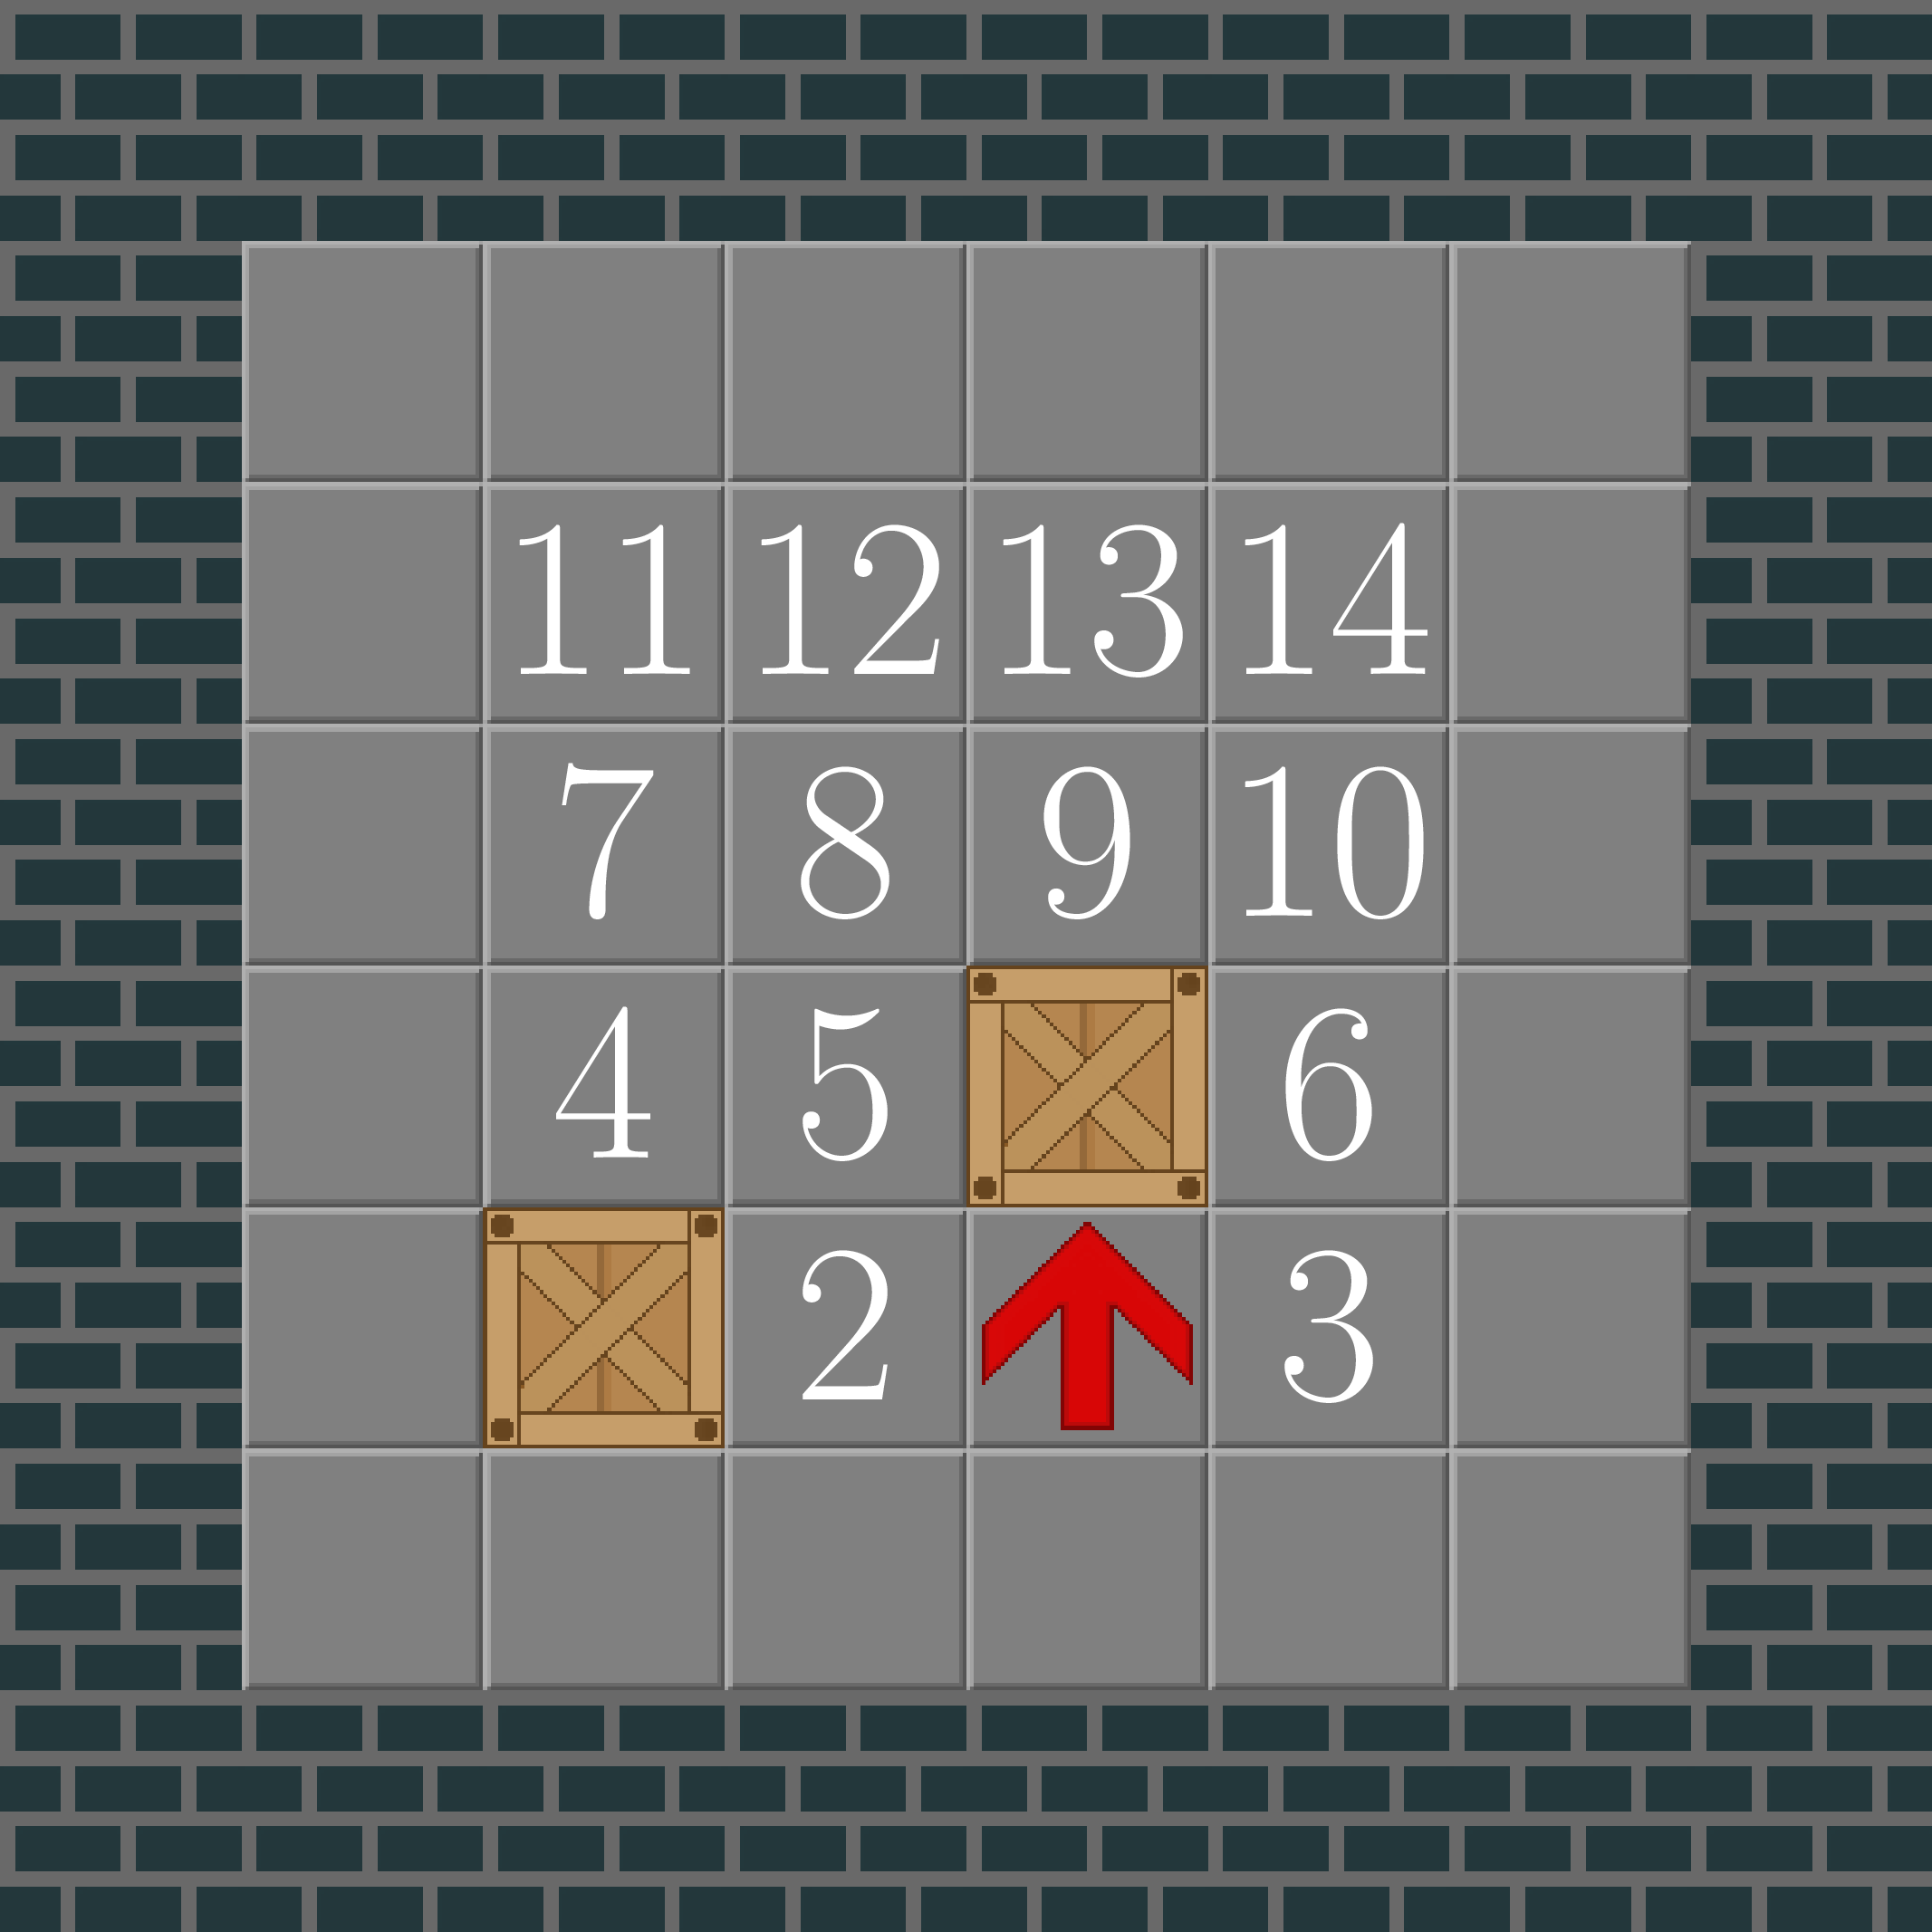
\includegraphics[width=0.2\textwidth]{tiles/crate.png} &
                    
\includegraphics[width=0.2\textwidth]{tiles/target.png} &
                    
\includegraphics[width=0.2\textwidth]{tiles/crate_on_target.png} \\
                   \textbf{Mur} & Sol & \textbf{Caisse} & Cible & \textbf{Caisse sur une cible} \\
                \end{tabular}
            }
        \end{frame}

        \begin{frame}{Problématique et réalisation}
            \centering
            \Large\textbf{Quelles stratégies adopter pour trouver une solution le plus rapidement possible à un niveau de Sokoban ?}

            \vspace{1.5cm} % don't remove the blank line above, otherwise it won't work (cf https://tex.stackexchange.com/a/204990)
            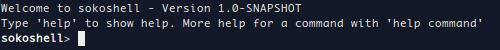
\includegraphics[width=\textwidth]{shell.png}
         \end{frame}

        \begin{frame}{Plan}
            \tableofcontents%[hideallsubsections]
        \end{frame}

        \begin{frame}{Lien avec le thème de l'année}
            \centering
            \only<1>{
                 \copyrightbox[b]{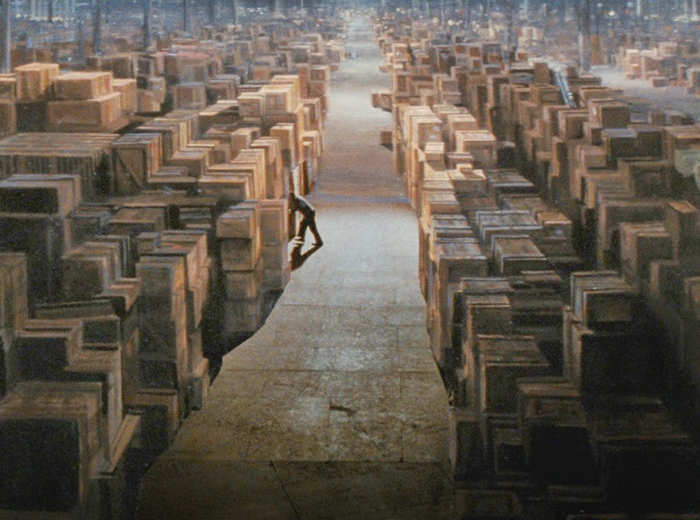
\includegraphics[width=0.9\textwidth]{warehouse.jpg}}
                                 {Source : \textit{Indiana Jones et les Aventuriers de l'arche perdue} (scène de fin), Steven Spielberg, 1981
                                          \url{https://pbs.twimg.com/media/EyjVShEVEAAQZjK.jpg}}%
            }
            \only<2>{
                \copyrightbox[b]{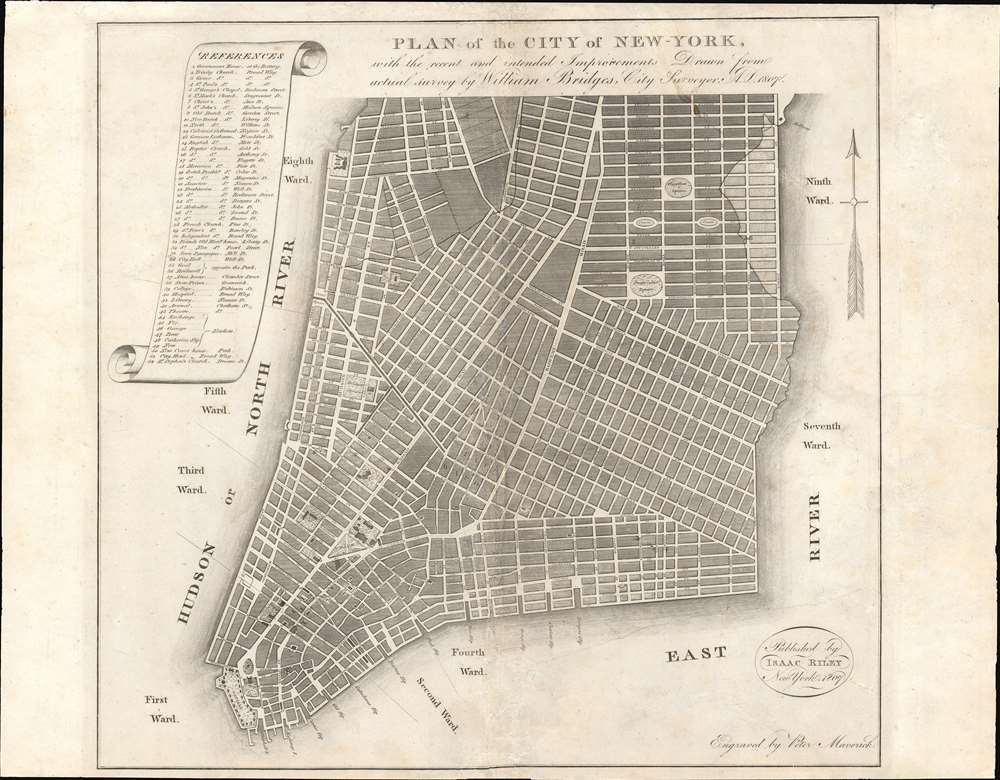
\includegraphics[width=0.9\textwidth]{city_plan.jpg}}
                                {Source : \url{https://www.geographicus.com/mm5/graphics/00000001/L/NewYork-bridgesmaverick-1807.jpg}}%
            }
        \end{frame}

    \section{Principe de résolution}
        \begin{frame}{Arbre des états}
            \begin{center}
    \begin{forest}
        for tree = {
            edge = {->}
        }
         [{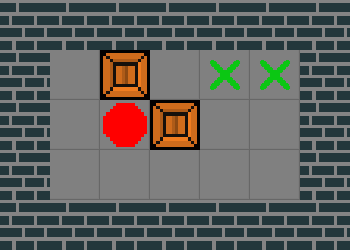
\includegraphics[width=0.3\textwidth]{search_tree/1.png}},
            [{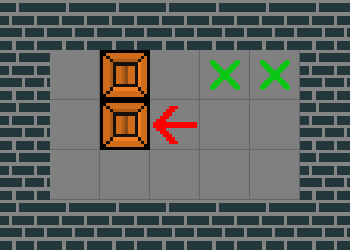
\includegraphics[width=0.3\textwidth]{search_tree/1_1.png}}, [...]]
            [...]
            [{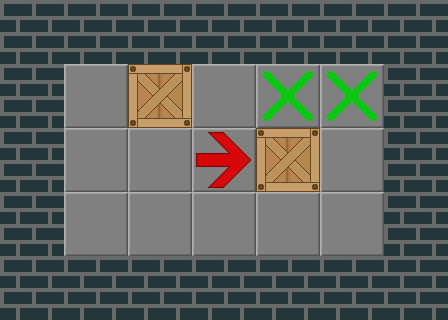
\includegraphics[width=0.3\textwidth]{search_tree/1_2.png}}, [...]]
        ]
    \end{forest}
\end{center}
        \end{frame}

        \begin{frame}{Calcul du \textit{hash} d'un état - Hash de Zobrist}
            \only<1>{
                Propriétés du \xor:
                \begin{enumerate}
                    \item $a \xor a = 0$
                    \item \xor commutatif, associatif
                    \item \xor préserve l'aléatoire
                \end{enumerate}

                Initialisation:

                \begin{center}
                    $T=\begin{blockarray}{ccc}
                            \text{caisse} & \text{joueur} & \text{case} \\
                        \begin{block}{(cc)c}
                            6357   & \candidatenumber   & 0      \\
                            -1378  & 42     & 1      \\
                            \vdots & \vdots & \vdots \\
                            93268  & -278   & wh - 1 \\
                        \end{block}
                    \end{blockarray}$
                \end{center}
            }

            \only<2>{
                \begin{itemize}
                    \item $(c_1, ..., c_n)$ $n$ caisses et $p$ position du joueur :
                        \[h = \underset{i=0}{\overset{n}{\xor}} T[c_i][0] \xor T[p][1] \]
                        \[\text{ en } \mathcal{O}(n)\]
                    \item \textbf{Connaissant le hash de l'état parent}: $c_i \rightarrow c_i', p \rightarrow p'$
                          \[h' = h \xor T[c_i][0] \xor T[c_i'][0] \xor T[p][1] \xor T[p'][1]\]
                          \[\boxed{\text{en }\mathcal{O}(1)}\]
                \end{itemize}
            }
        \end{frame}

    \section{Réduction de l'espace de recherche}

        \subsection{Analyse statique}

            \begin{frame}{Détection des positions mortes \textit{(dead tiles)}}
                \centering

                \resizebox{\textwidth}{!}{%
                    \begin{tikzpicture}
                        \node {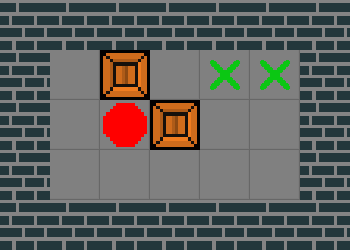
\includegraphics[width=0.7\textwidth]{dead_positions/example_after.png}};
                    \end{tikzpicture}
                }
            \end{frame}

            \begin{interstateframe}
                \begin{interstatenv}{1}{0}\interstatplot{1};\end{interstatenv}
            \end{interstateframe}

            \begin{frame}{Détection de tunnels}
                \includegraphics<1>[width=\textwidth]{tunnels/tunnels.png}%
                \only<2>{
                    \begin{center}
                        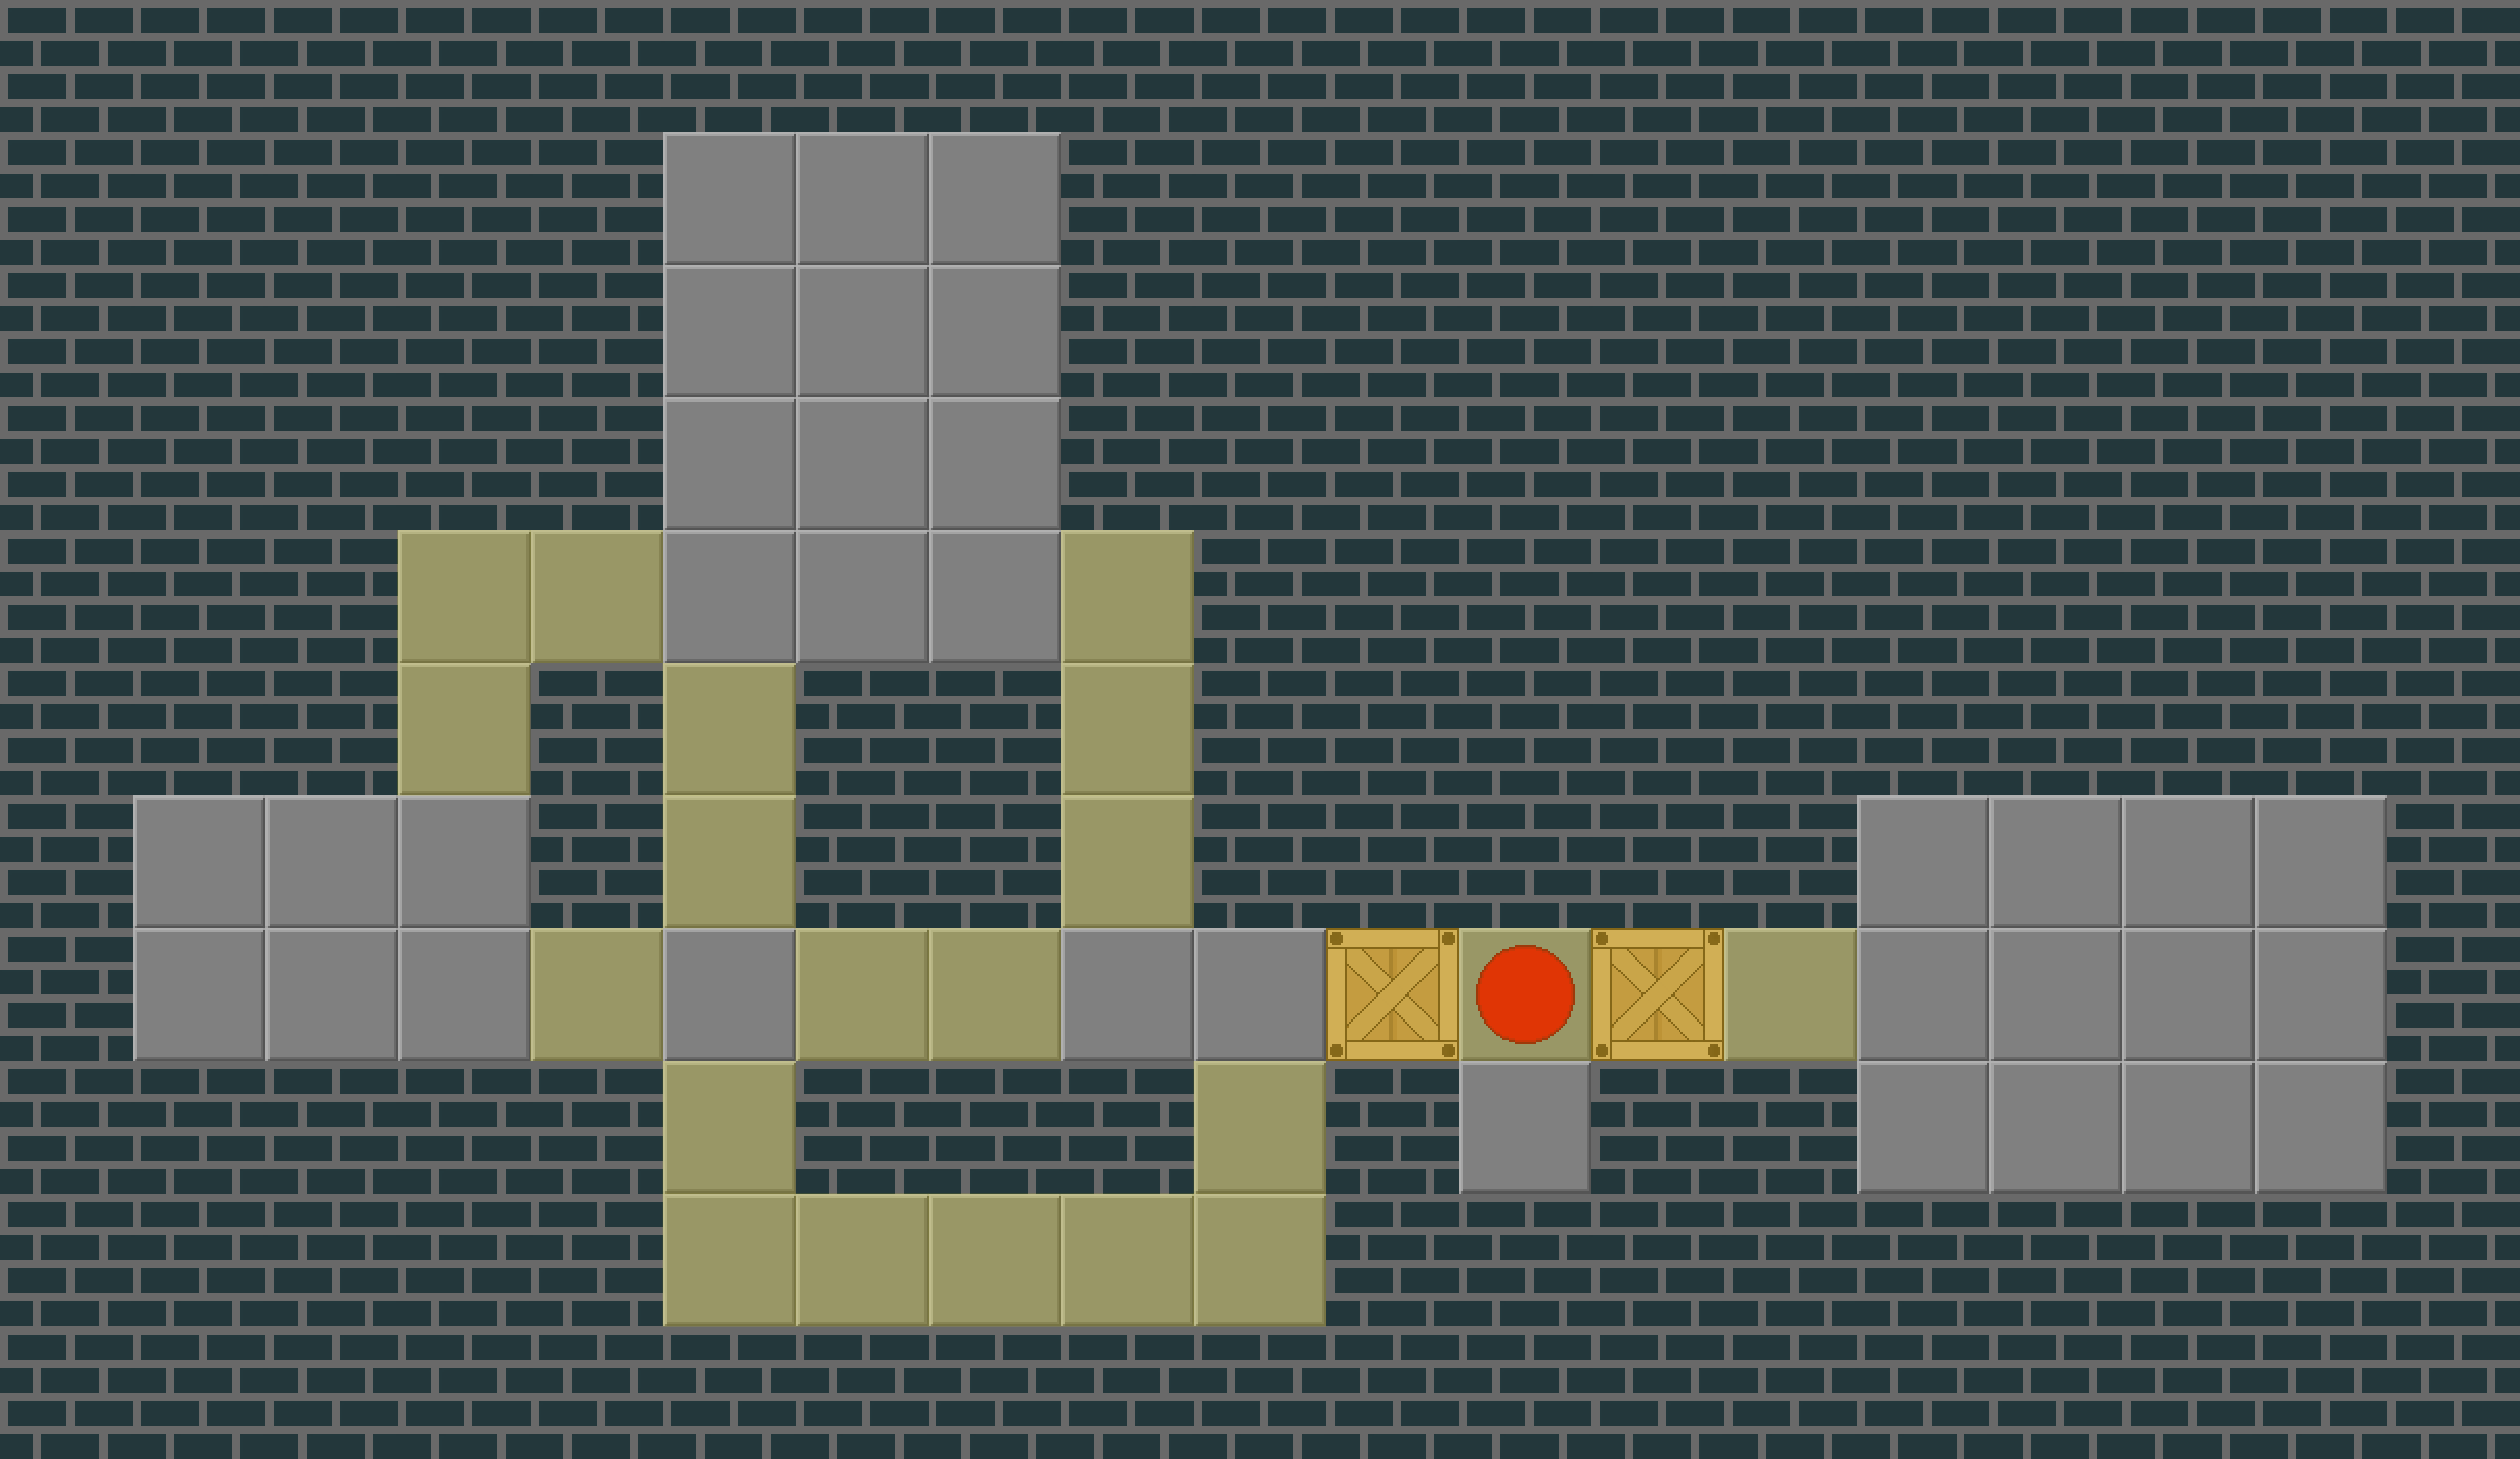
\includegraphics[width=0.58\textwidth]{tunnels/tunnel_macro_one_crate_1.png}

                        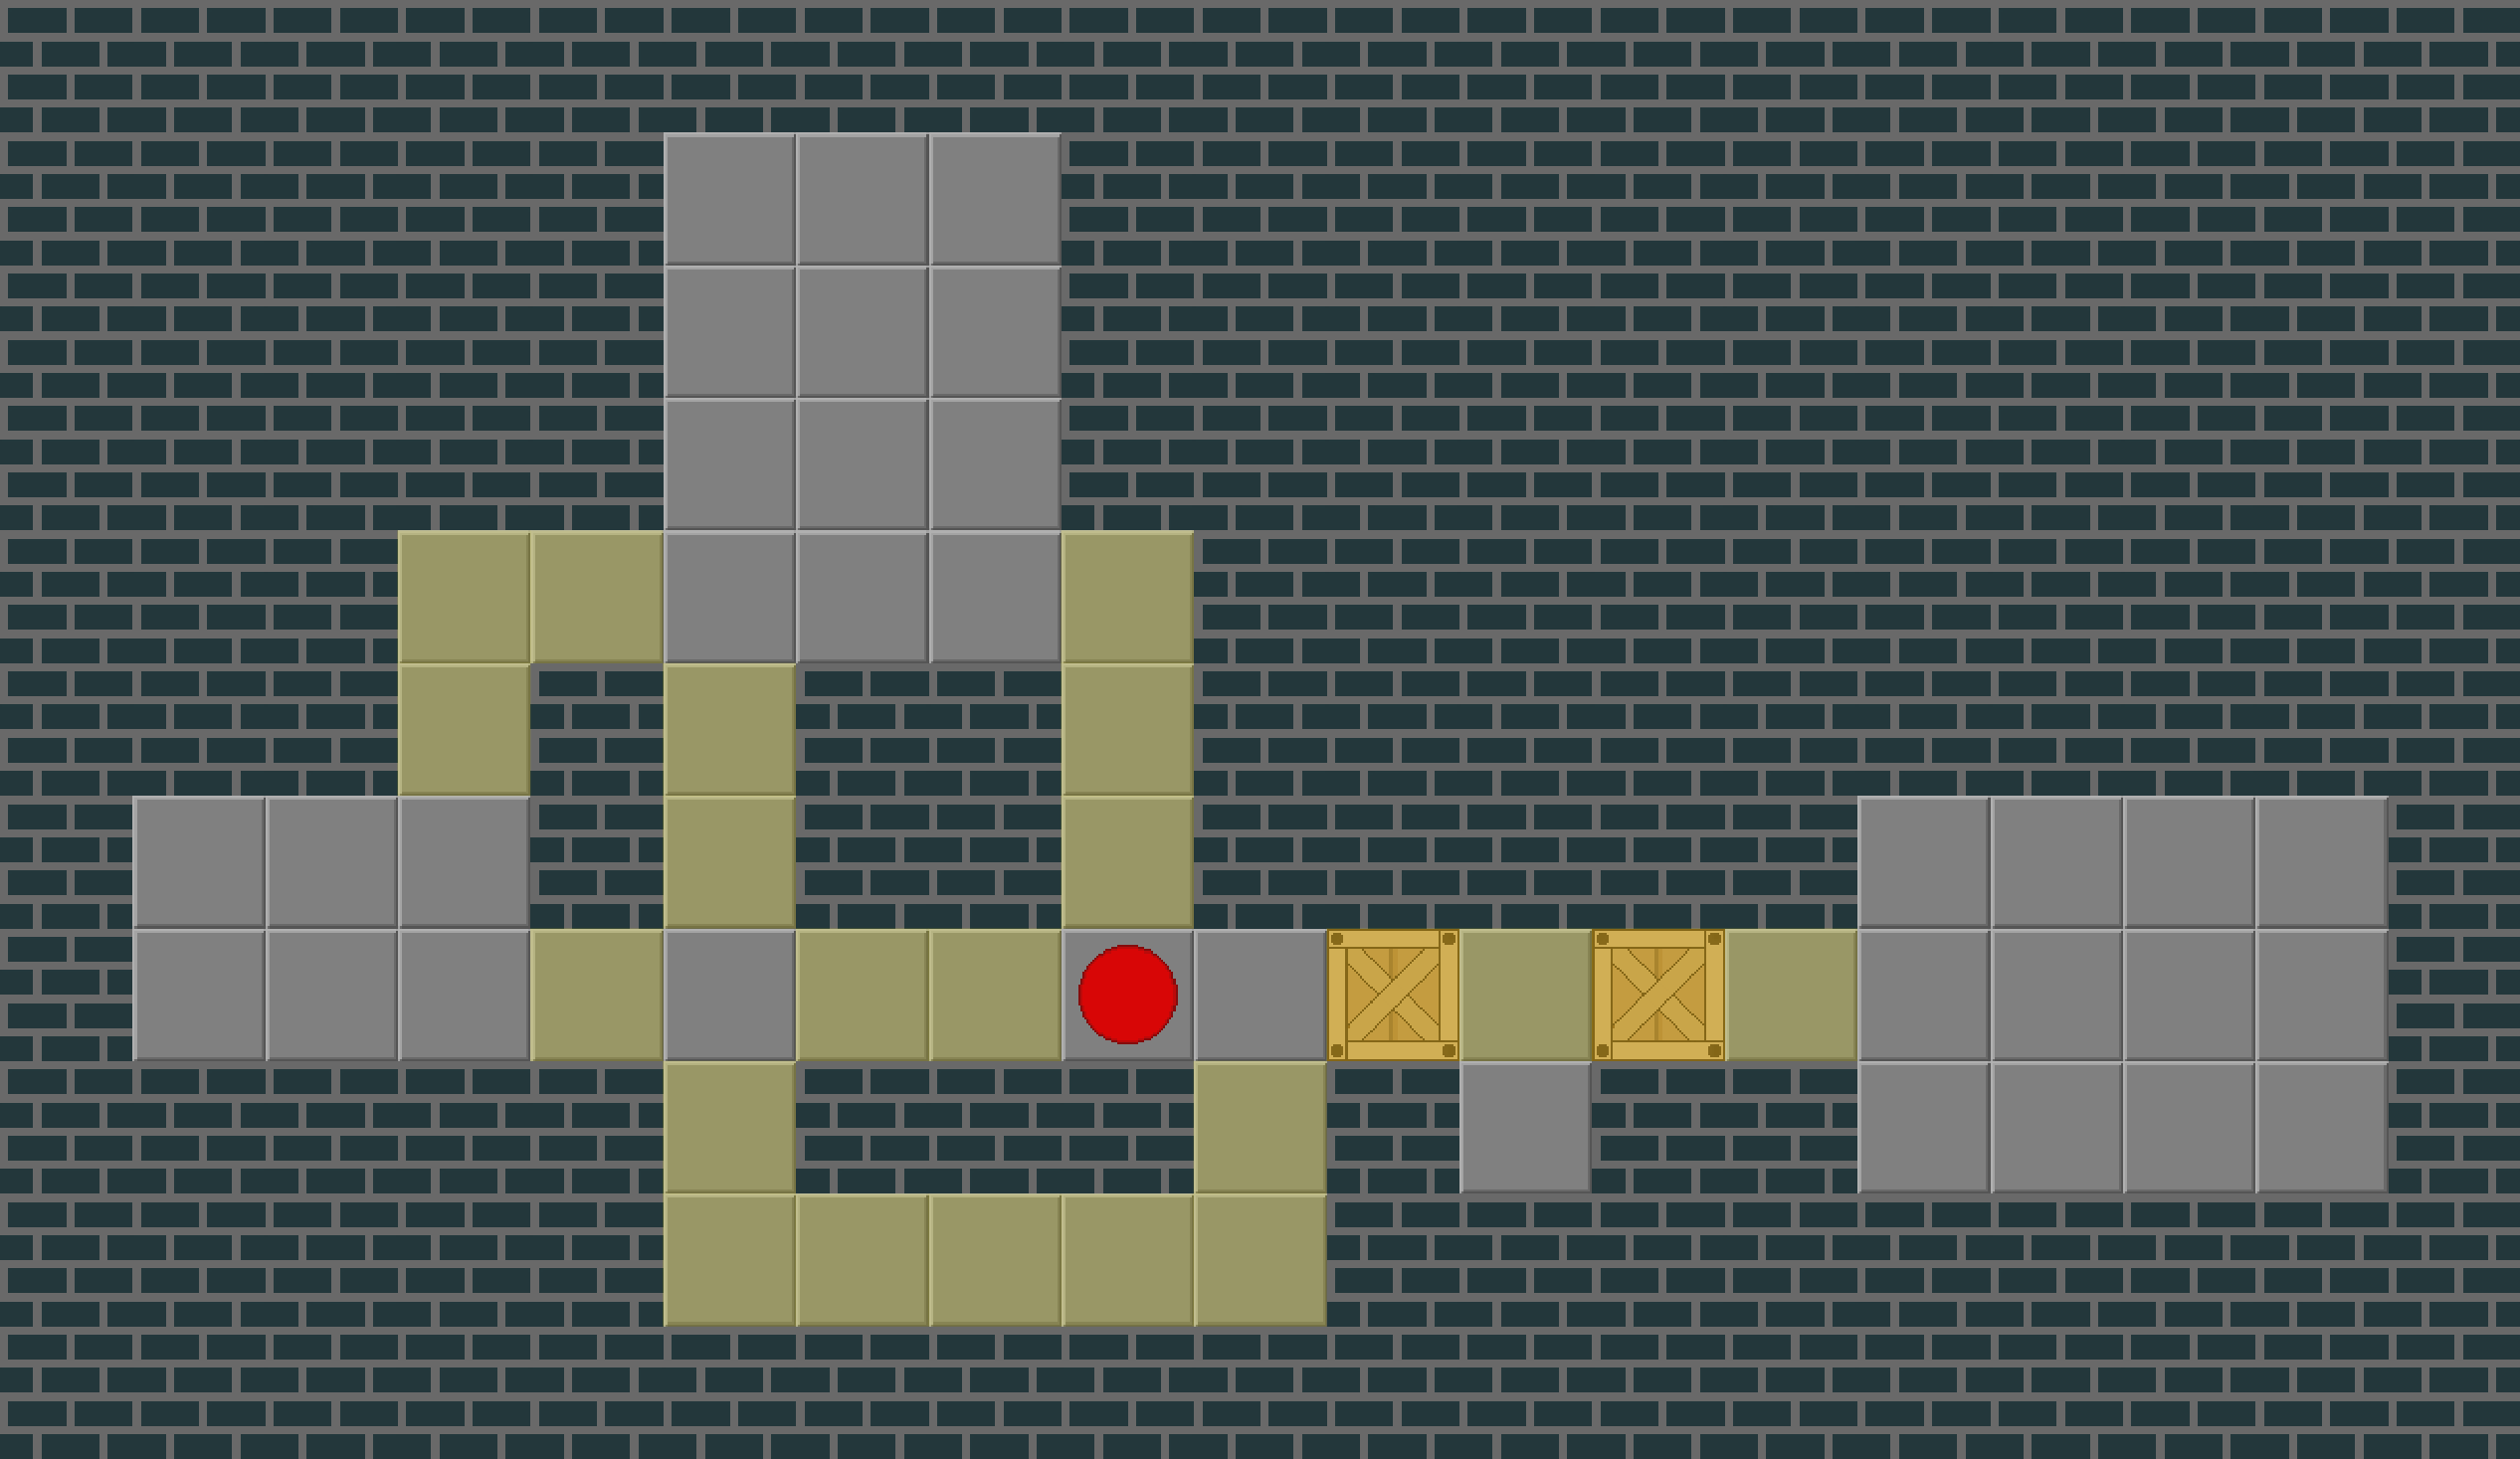
\includegraphics[width=0.58\textwidth]{tunnels/tunnel_macro_one_crate_2.png}
                    \end{center}
                }
                \includegraphics<3>[width=\textwidth]{tunnels/tunnel_macro.png}%
                \includegraphics<4>[width=\textwidth]{tunnels/tunnel_macro_player_only.png}%
                \includegraphics<5>[width=\textwidth]{tunnels/tunnel_macro_oneway.png}%
                \only<6>{
                    \begin{minipage}{0.4\textwidth}
                         
\includegraphics[width=\textwidth]{tunnels/straight.png}
                    \end{minipage}
                    \hfill
                    \begin{minipage}{0.4\textwidth}
                         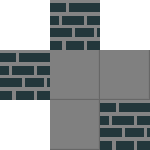
\includegraphics[width=\textwidth]{tunnels/corner.png}
                    \end{minipage}

                    \centering
                    Composition d'un tunnel
                }
            \end{frame}

            \begin{interstateframe}
                \begin{interstatenv}{1}{0}\interstatplot{2};\end{interstatenv}
            \end{interstateframe}

            \begin{frame}{Salles et ordre de rangement \textit{(packing order)}}
                \centering
                \only<1>{
                    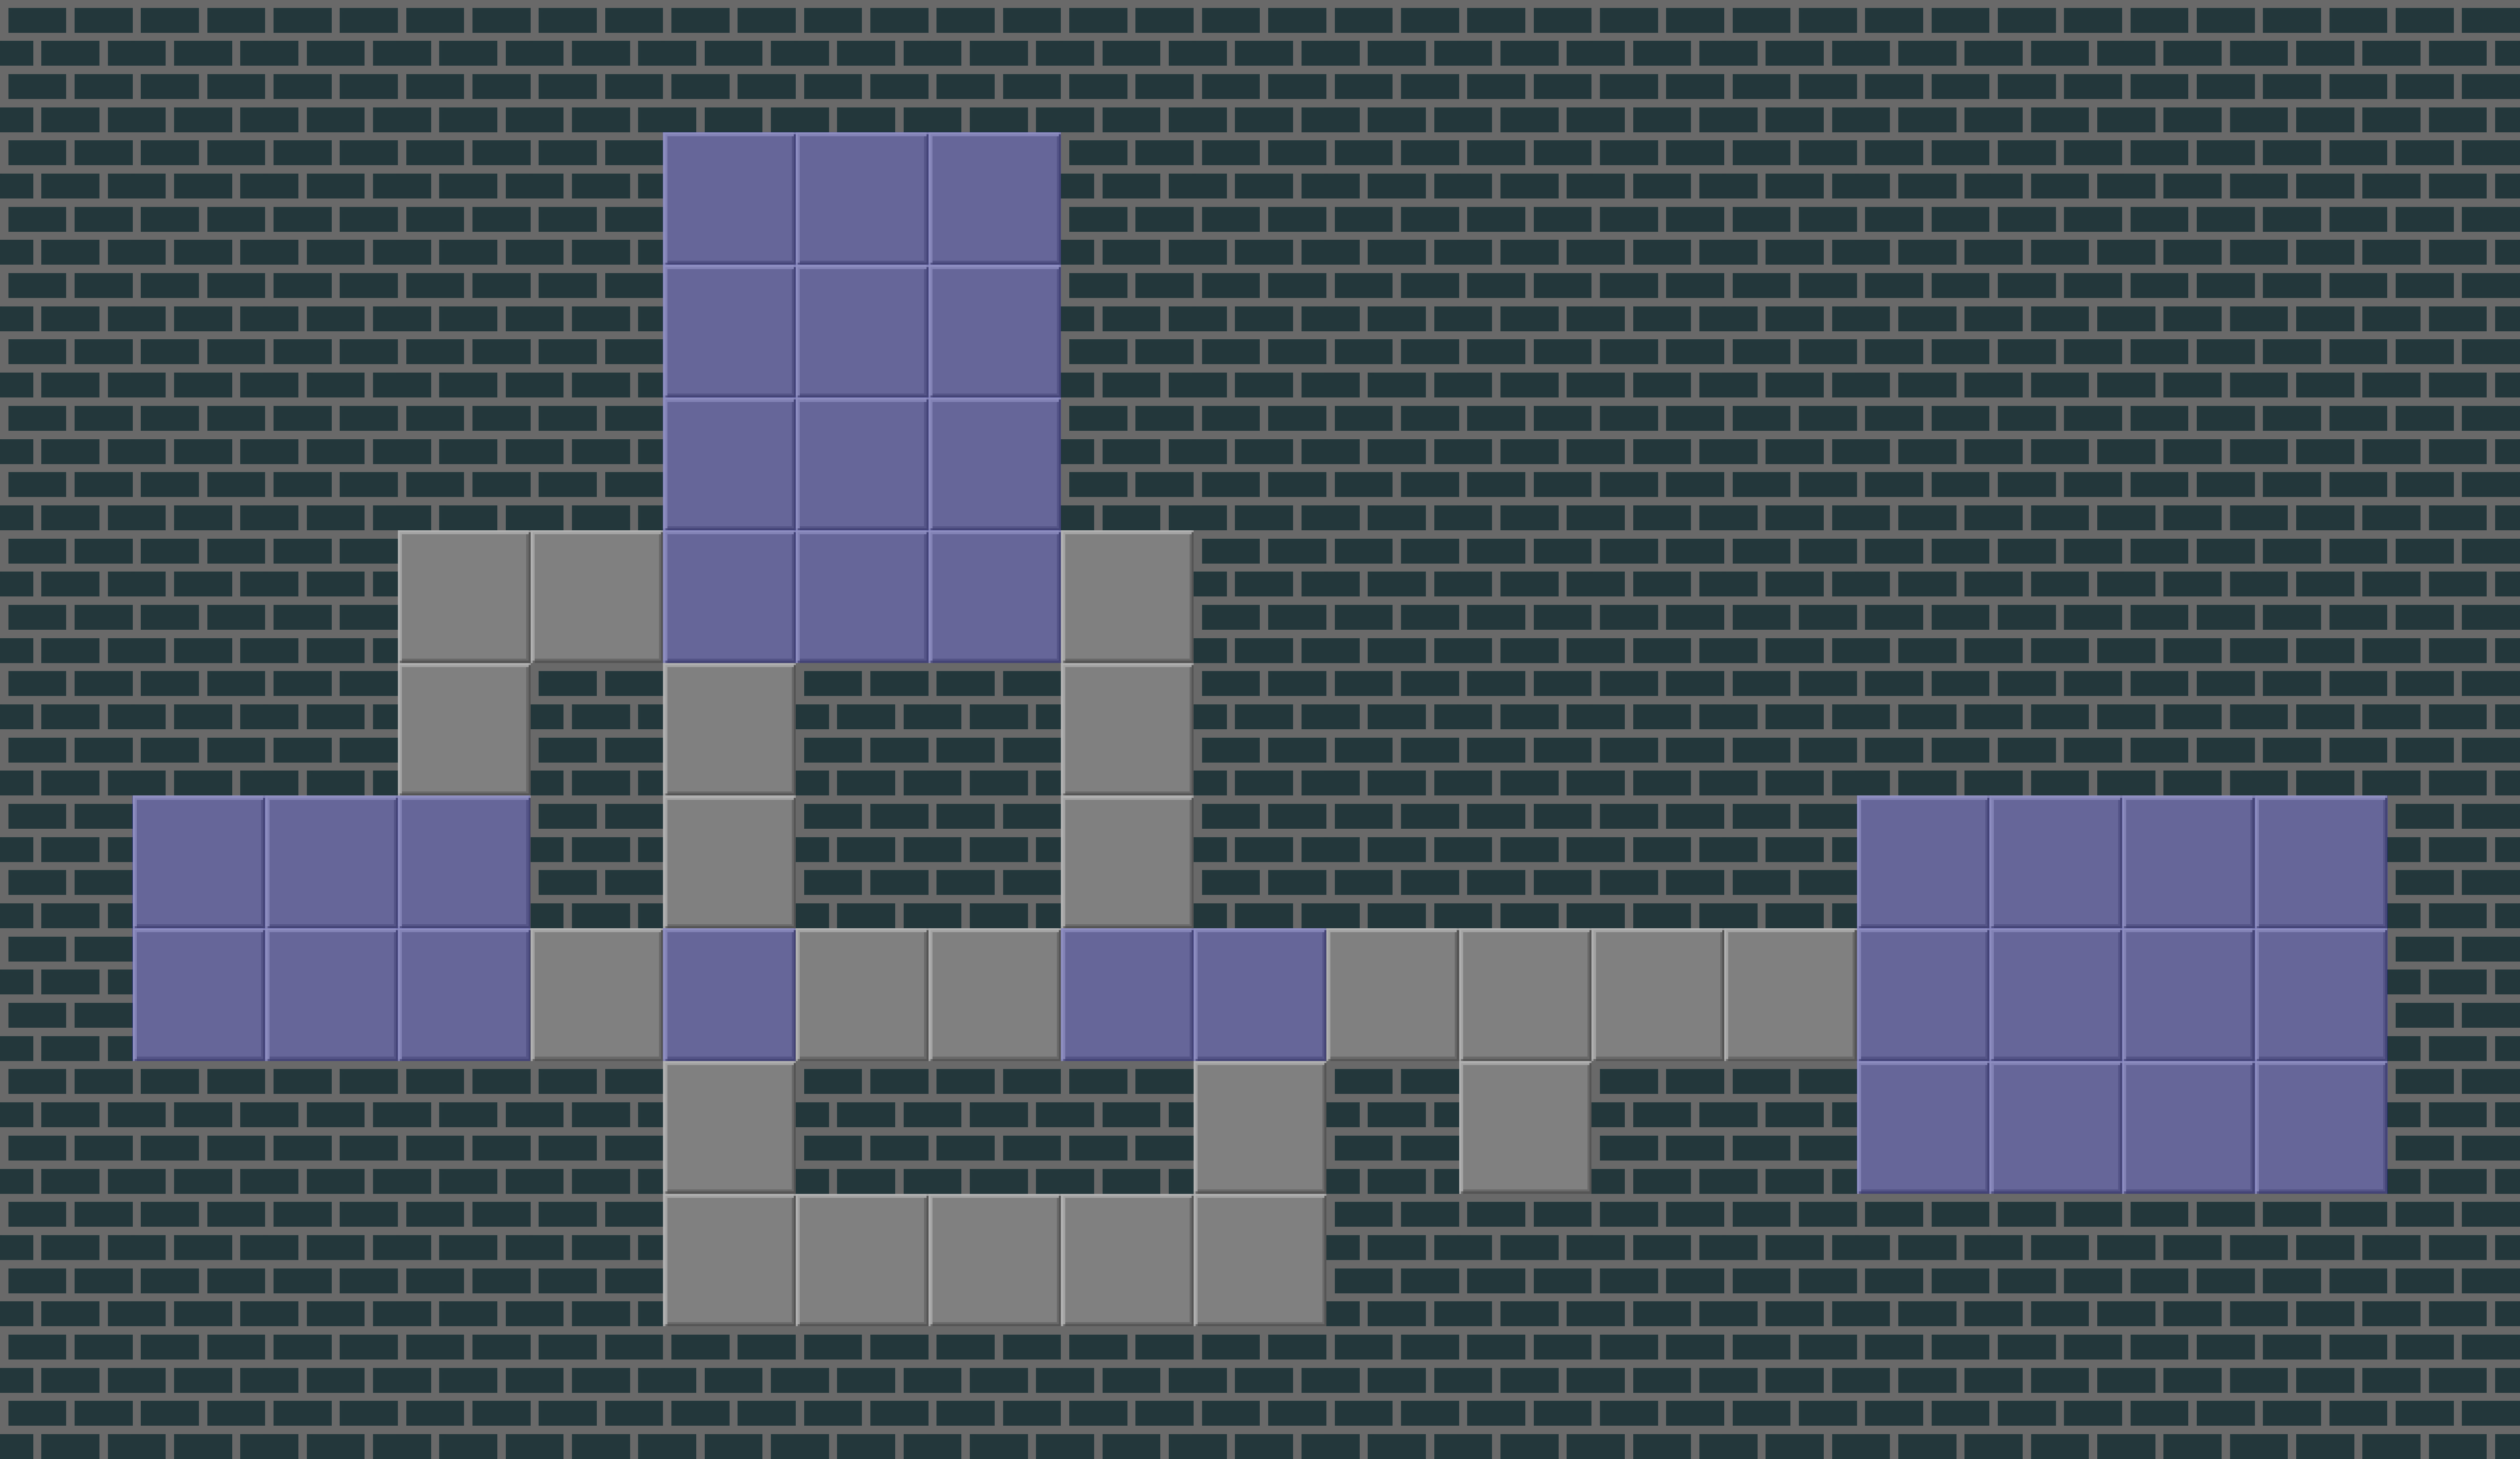
\includegraphics[width=\textwidth]{rooms_packing_order/rooms.png}
                }
                \only<2>{
                    \begin{tikzpicture}
                        \node (A) {
                            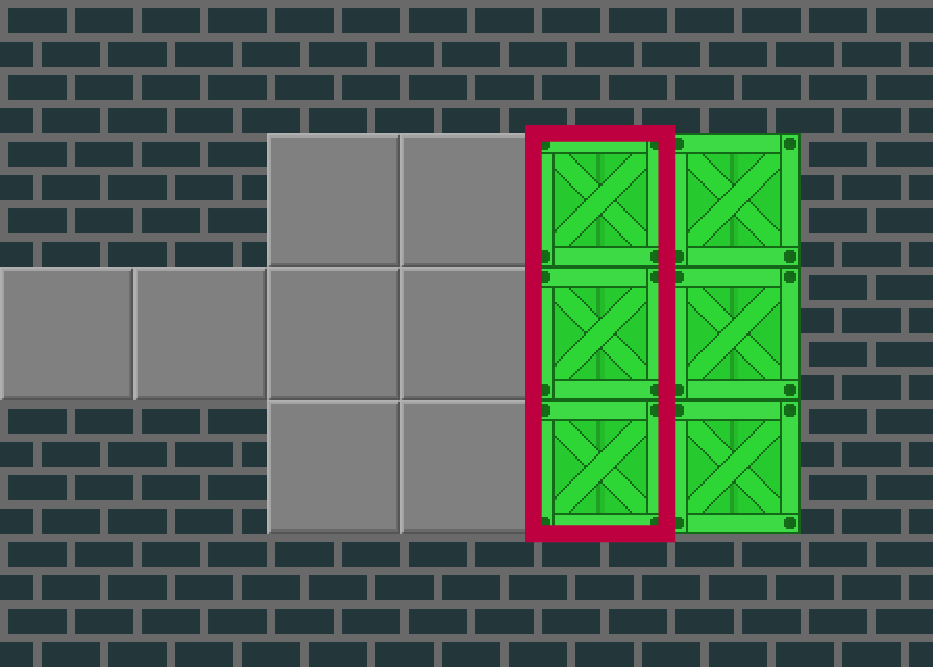
\includegraphics[width=0.4\textwidth]{rooms_packing_order/algo_1.png}
                        };
                        \node[right=of A] (B) {
                            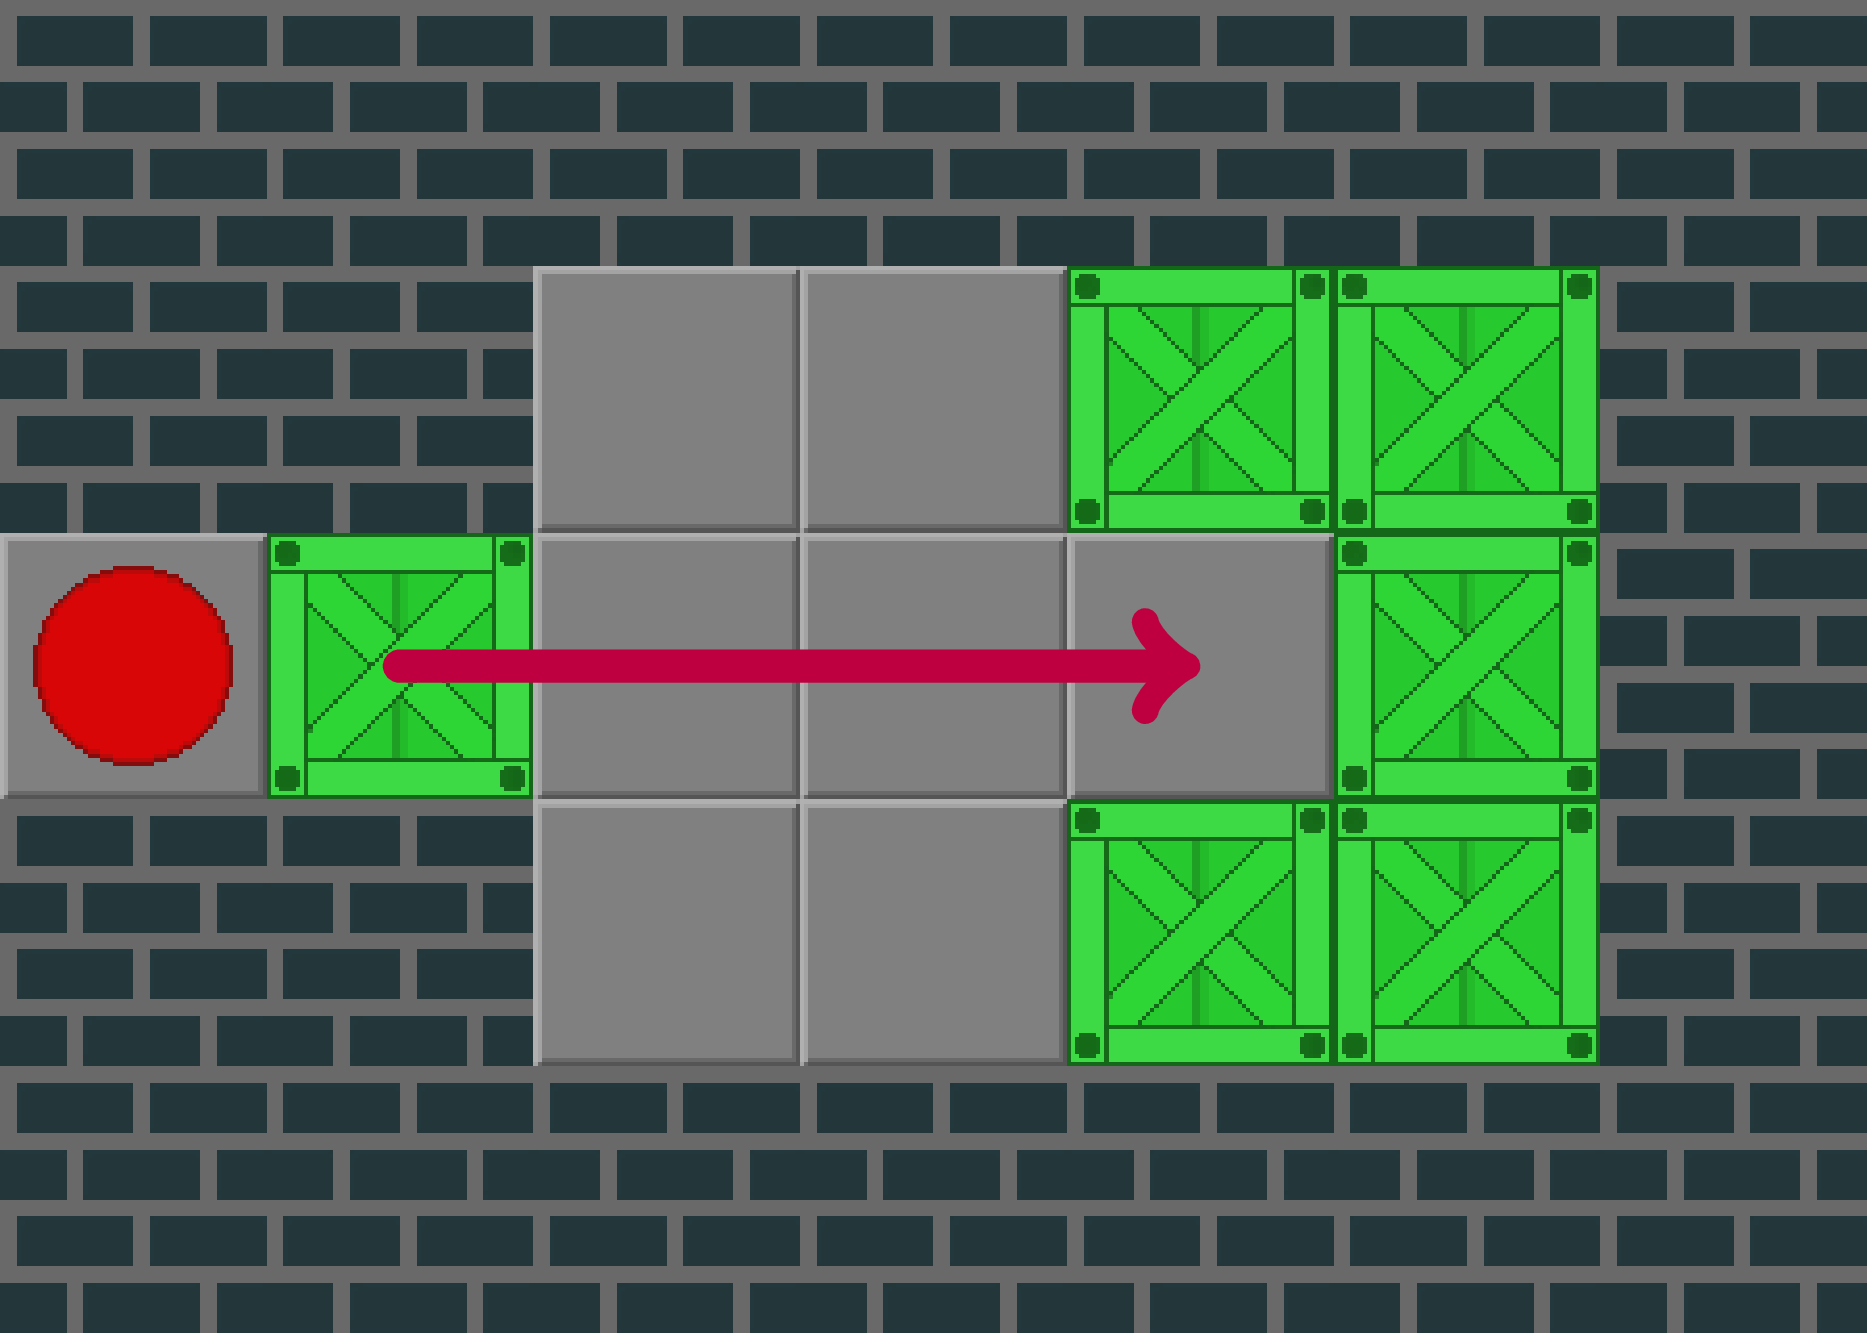
\includegraphics[width=0.4\textwidth]{rooms_packing_order/algo_2.png}
                        };
                        \node[below=of A] (C) {
                            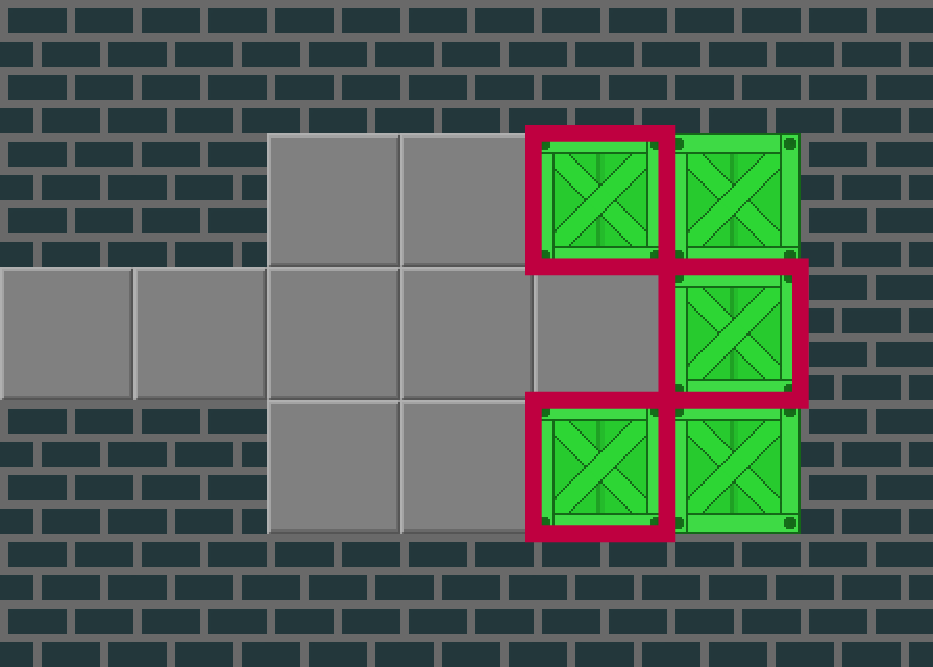
\includegraphics[width=0.4\textwidth]{rooms_packing_order/algo_3.png}
                        };
                        \node[below=of B] (D) {
                            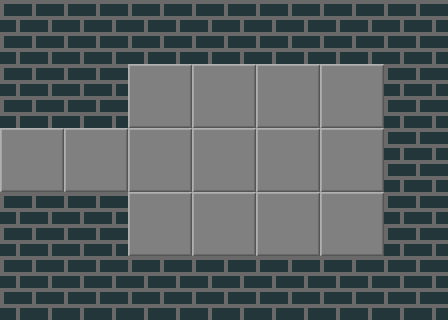
\includegraphics[width=0.4\textwidth]{rooms_packing_order/algo_4.png}
                        };

                        \draw[->, line width=\arrowwidth] (A.east) -- (B.west);

                        \coordinate (I) at ($ (B) ! .5 ! (C) $);
                        \draw[->, line width=\arrowwidth] (B.south) |- (I) -| (C.north);
                        \draw[->, line width=\arrowwidth, dashed] (C.east) -- (D.west);
                    \end{tikzpicture}
                }
                \only<3>{
                    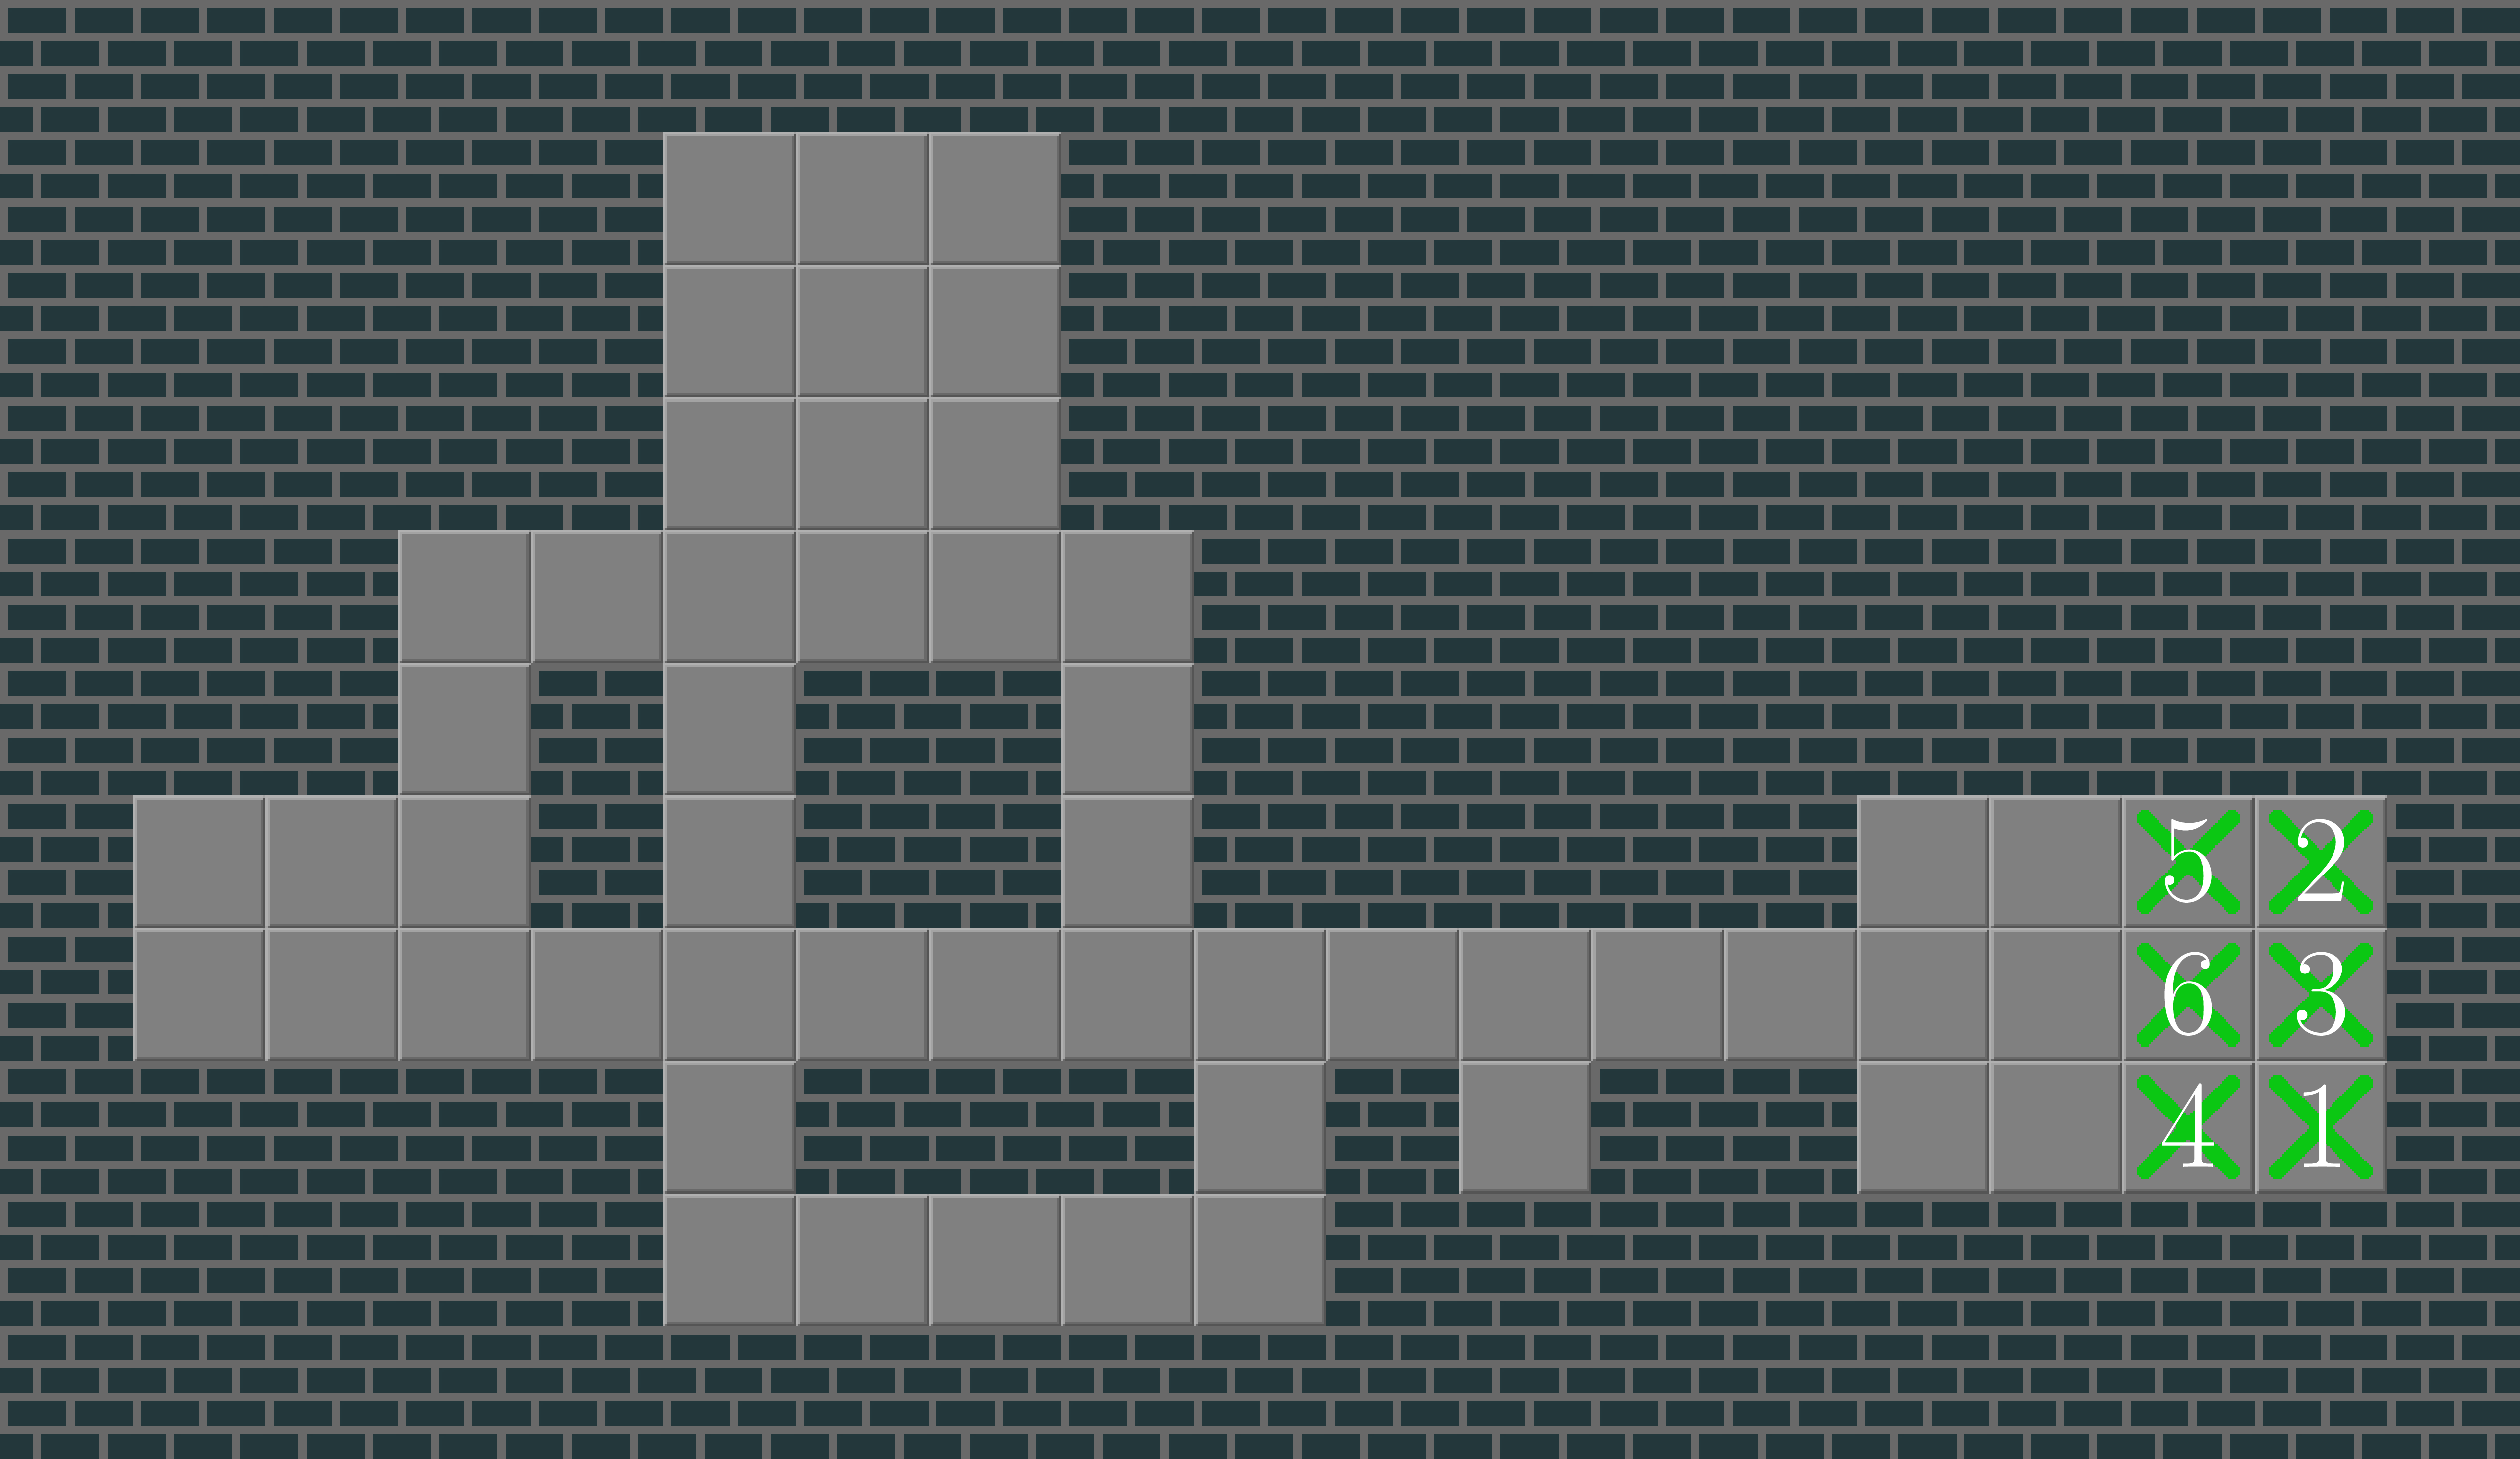
\includegraphics[width=\textwidth]{rooms_packing_order/packing_order.png}
                }
                \only<4>{
                    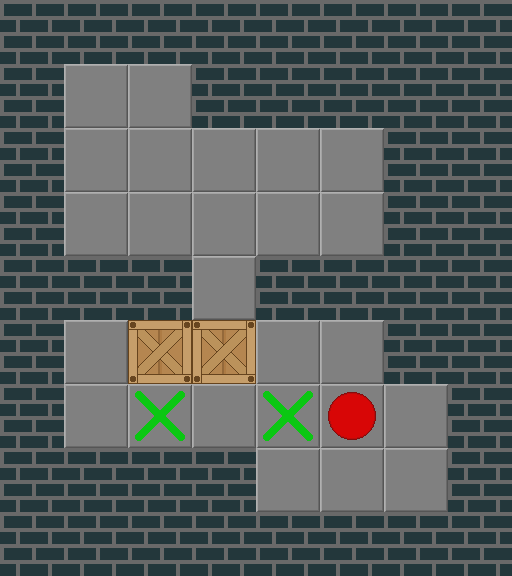
\includegraphics[height=0.8\textheight]{rooms_packing_order/no_packing_order.png}
                }
            \end{frame}

            \begin{interstateframe}
                \begin{interstatenv}{1}{0}\interstatplot{3};\end{interstatenv}
            \end{interstateframe}

        \subsection{Analyse dynamique}

            \begin{frame}{Détection d'impasses \textit{(deadlocks)}}
                \begin{figure}
                    \centering
                    \subcaptionbox{\textit{Freeze deadlock n°1}} {
                        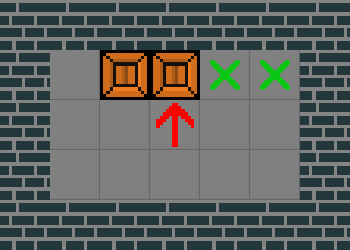
\includegraphics[width=0.4\textwidth]{freeze_deadlock/ex_1_dead.png}
                    }
                    \subcaptionbox{\textit{Freeze deadlock n°2}} {
                        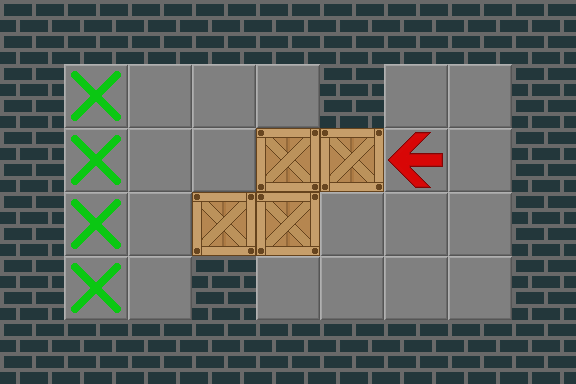
\includegraphics[width=0.4\textwidth]{freeze_deadlock/ex_2_dead.png}
                    }
                    \subcaptionbox{\textit{PI Corral deadlock}} {
                        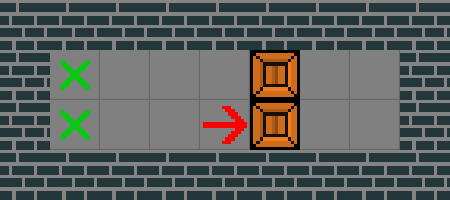
\includegraphics[width=0.4\textwidth]{pi_corral_deadlock_dead.png}
                    }
                \end{figure}
            \end{frame}

            \begin{frame}{Détection de \textit{freeze deadlocks}}
                \begin{figure}
                    \subcaptionbox{\textit{Règle n°1}} {
                        
\includegraphics[width=0.3\textwidth]{freeze_deadlock/rule_1.png}
                    }
                    \subcaptionbox{\textit{Règle n°2}} {
                        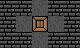
\includegraphics[width=0.3\textwidth]{freeze_deadlock/rule_2.png}
                    }
                    \subcaptionbox{\textit{Règle n°3}} {
                        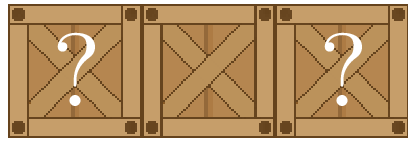
\includegraphics[width=0.3\textwidth]{freeze_deadlock/rule_3.png}
                    }
                \end{figure}
            \end{frame}

            \begin{frame}{Détection de \textit{freeze deadlocks}}
                \centering
                \begin{tikzpicture}
                    \node (start) {
                        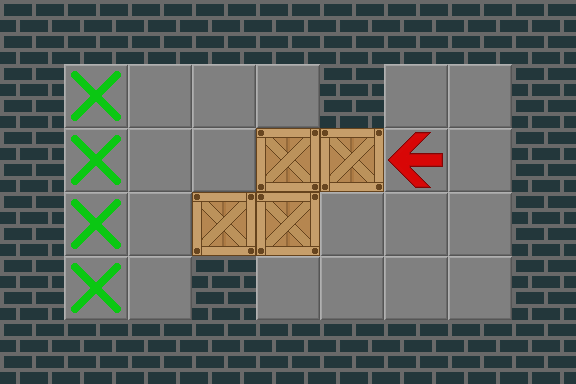
\includegraphics[width=0.4\textwidth]{freeze_deadlock/ex_2_dead.png}
                    };
                    \node[visible on=<2-4>, right=of start] (first) {
                        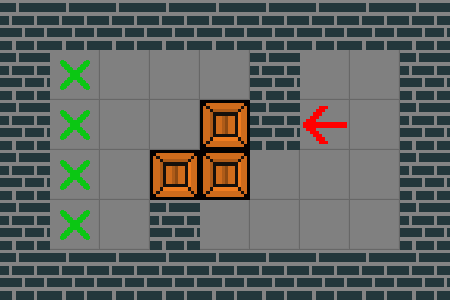
\includegraphics[width=0.4\textwidth]{freeze_deadlock/ex_2_explanation_1.png}
                    };
                    \node[visible on=<3-4>, below=of first] (second) {
                        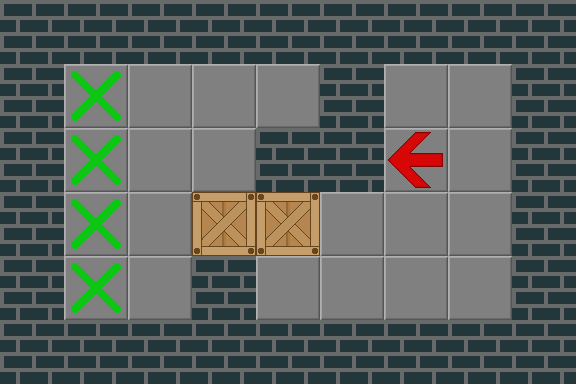
\includegraphics[width=0.4\textwidth]{freeze_deadlock/ex_2_explanation_2.png}
                    };
                    \node[visible on=<4>, left=of second] (third) {
                        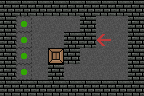
\includegraphics[width=0.4\textwidth]{freeze_deadlock/ex_2_explanation_3.png}
                    };
                    % don't remove '0cm', otherwise tikz will place the text too below
                    \node [visible on=<4>, below=0cm of third.south] {Gelée!};

                    \draw[->, line width=\arrowwidth, visible on=<2-4>] (start.east)  -- (first.west);
                    \draw[->, line width=\arrowwidth, visible on=<3-4>] (first.south) -- (second.north);
                    \draw[->, line width=\arrowwidth, visible on=<4>] (second.west) -- (third.east);
                \end{tikzpicture}
            \end{frame}

            \begin{interstateframe}
                \begin{interstatenv}{2}{1}\interstatplot{4};\end{interstatenv}
            \end{interstateframe}

            \begin{frame}{Détection de \textit{PI Corral deadlocks}}
                \only<1> {
                    \begin{minipage}{0.9\textwidth}
                        \begin{figure}
                            \centering
                            \subcaptionbox{\textit{Corral}} {
                                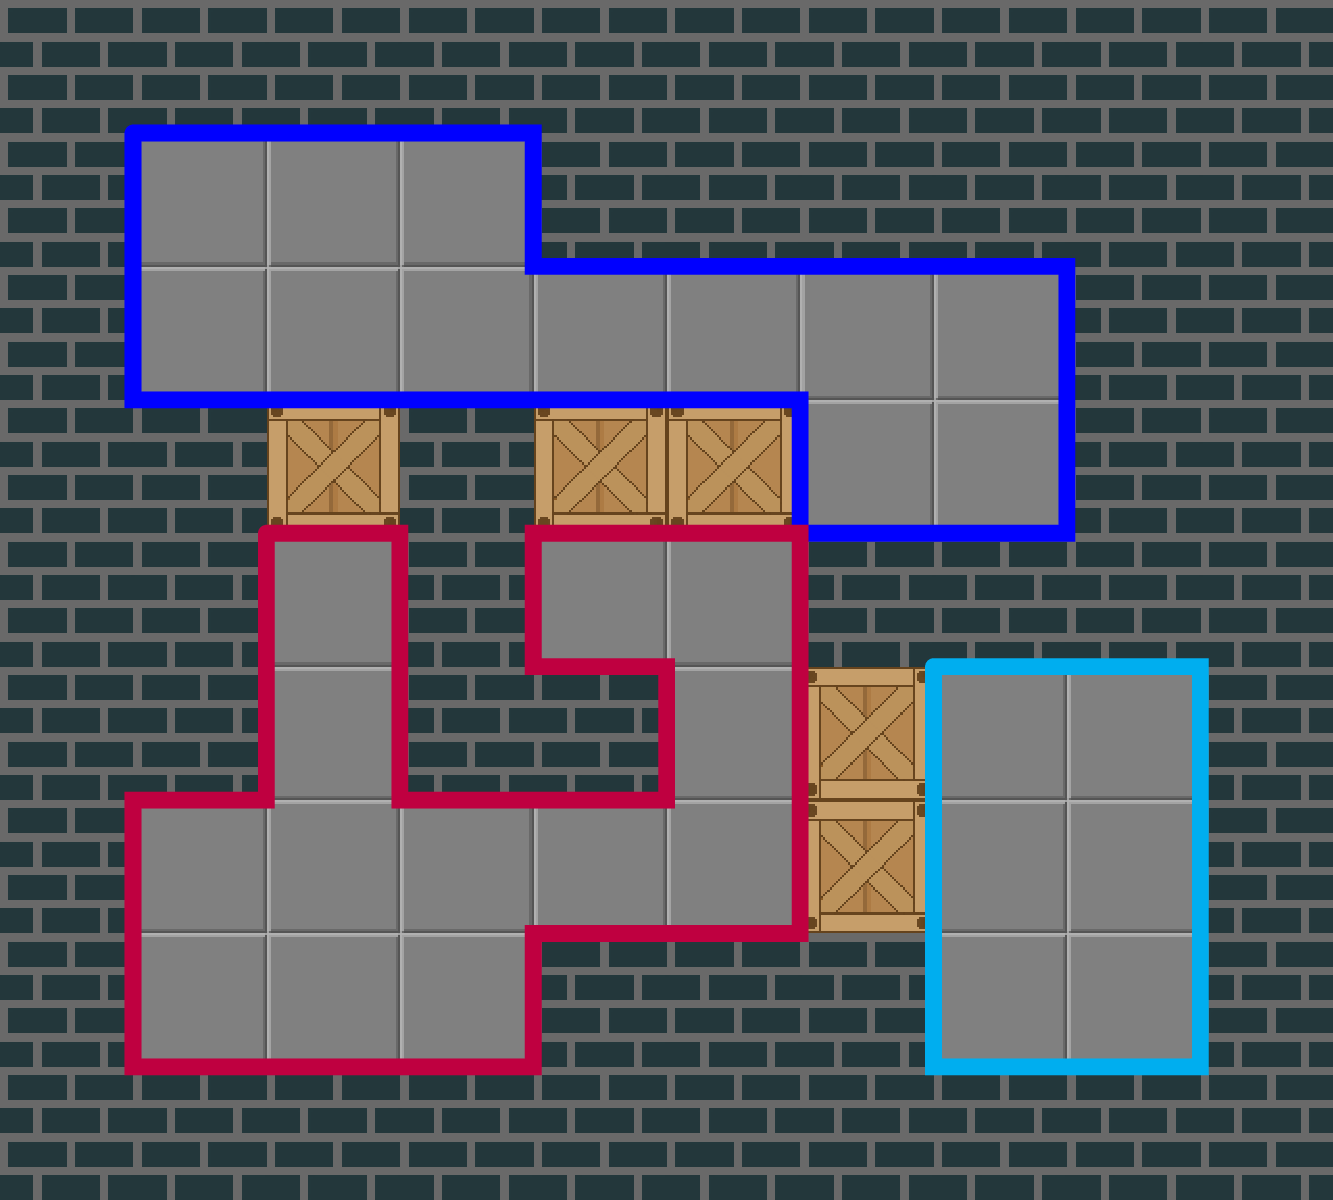
\includegraphics[width=0.4\textwidth]{corral/corral.png}%
                            }
                            \subcaptionbox{\textit{I Corral}} {
                                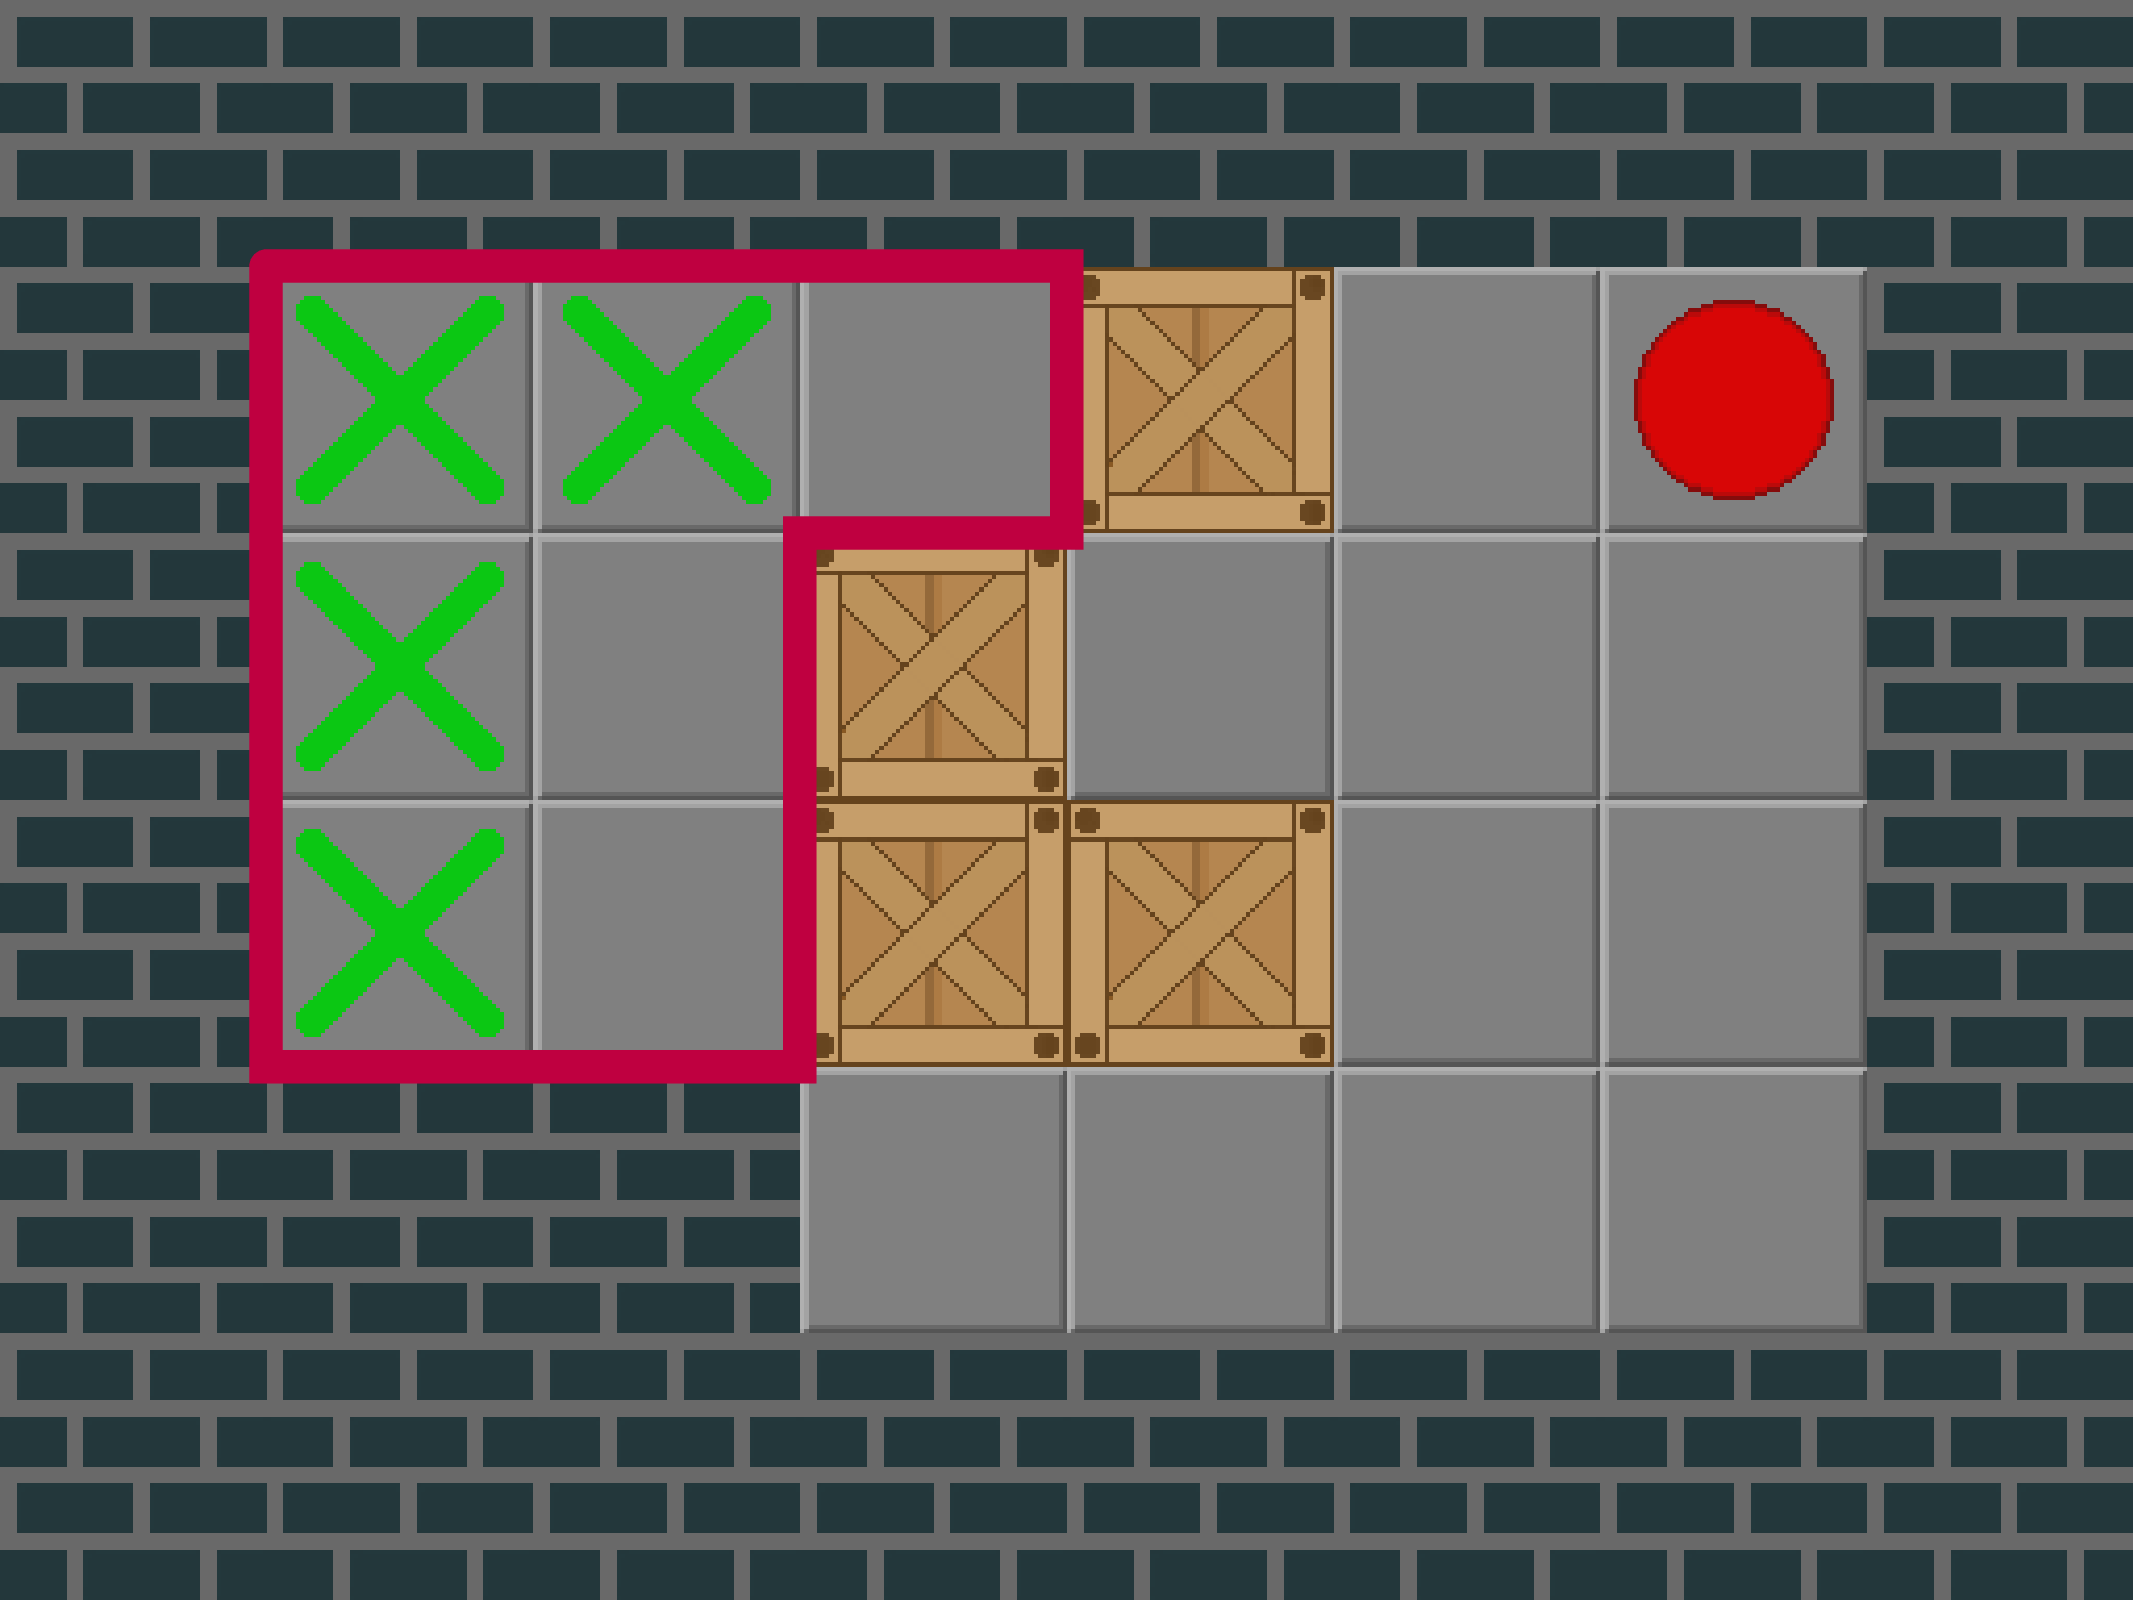
\includegraphics[width=0.4\textwidth]{corral/i_corral.png}%
                            }
                            \subcaptionbox{\textit{PI Corral}} {
                                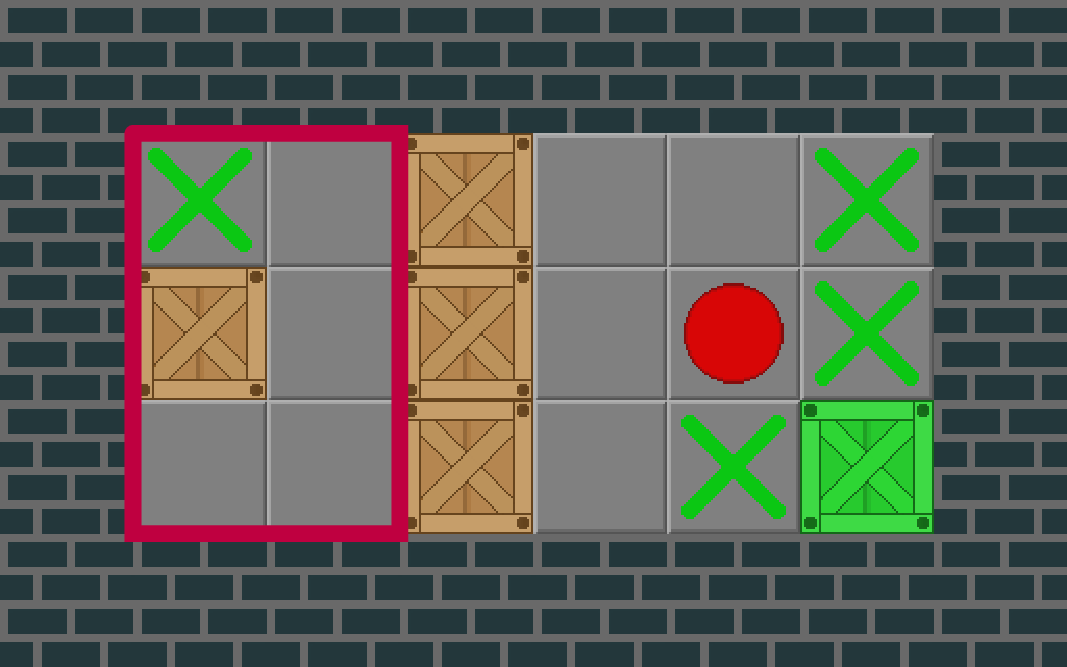
\includegraphics[width=0.4\textwidth]{corral/pi_corral.png}%
                            }
                        \end{figure}
                    \end{minipage}
                }
                \only<2>{
                    \begin{minipage}{0.45\textwidth}
                        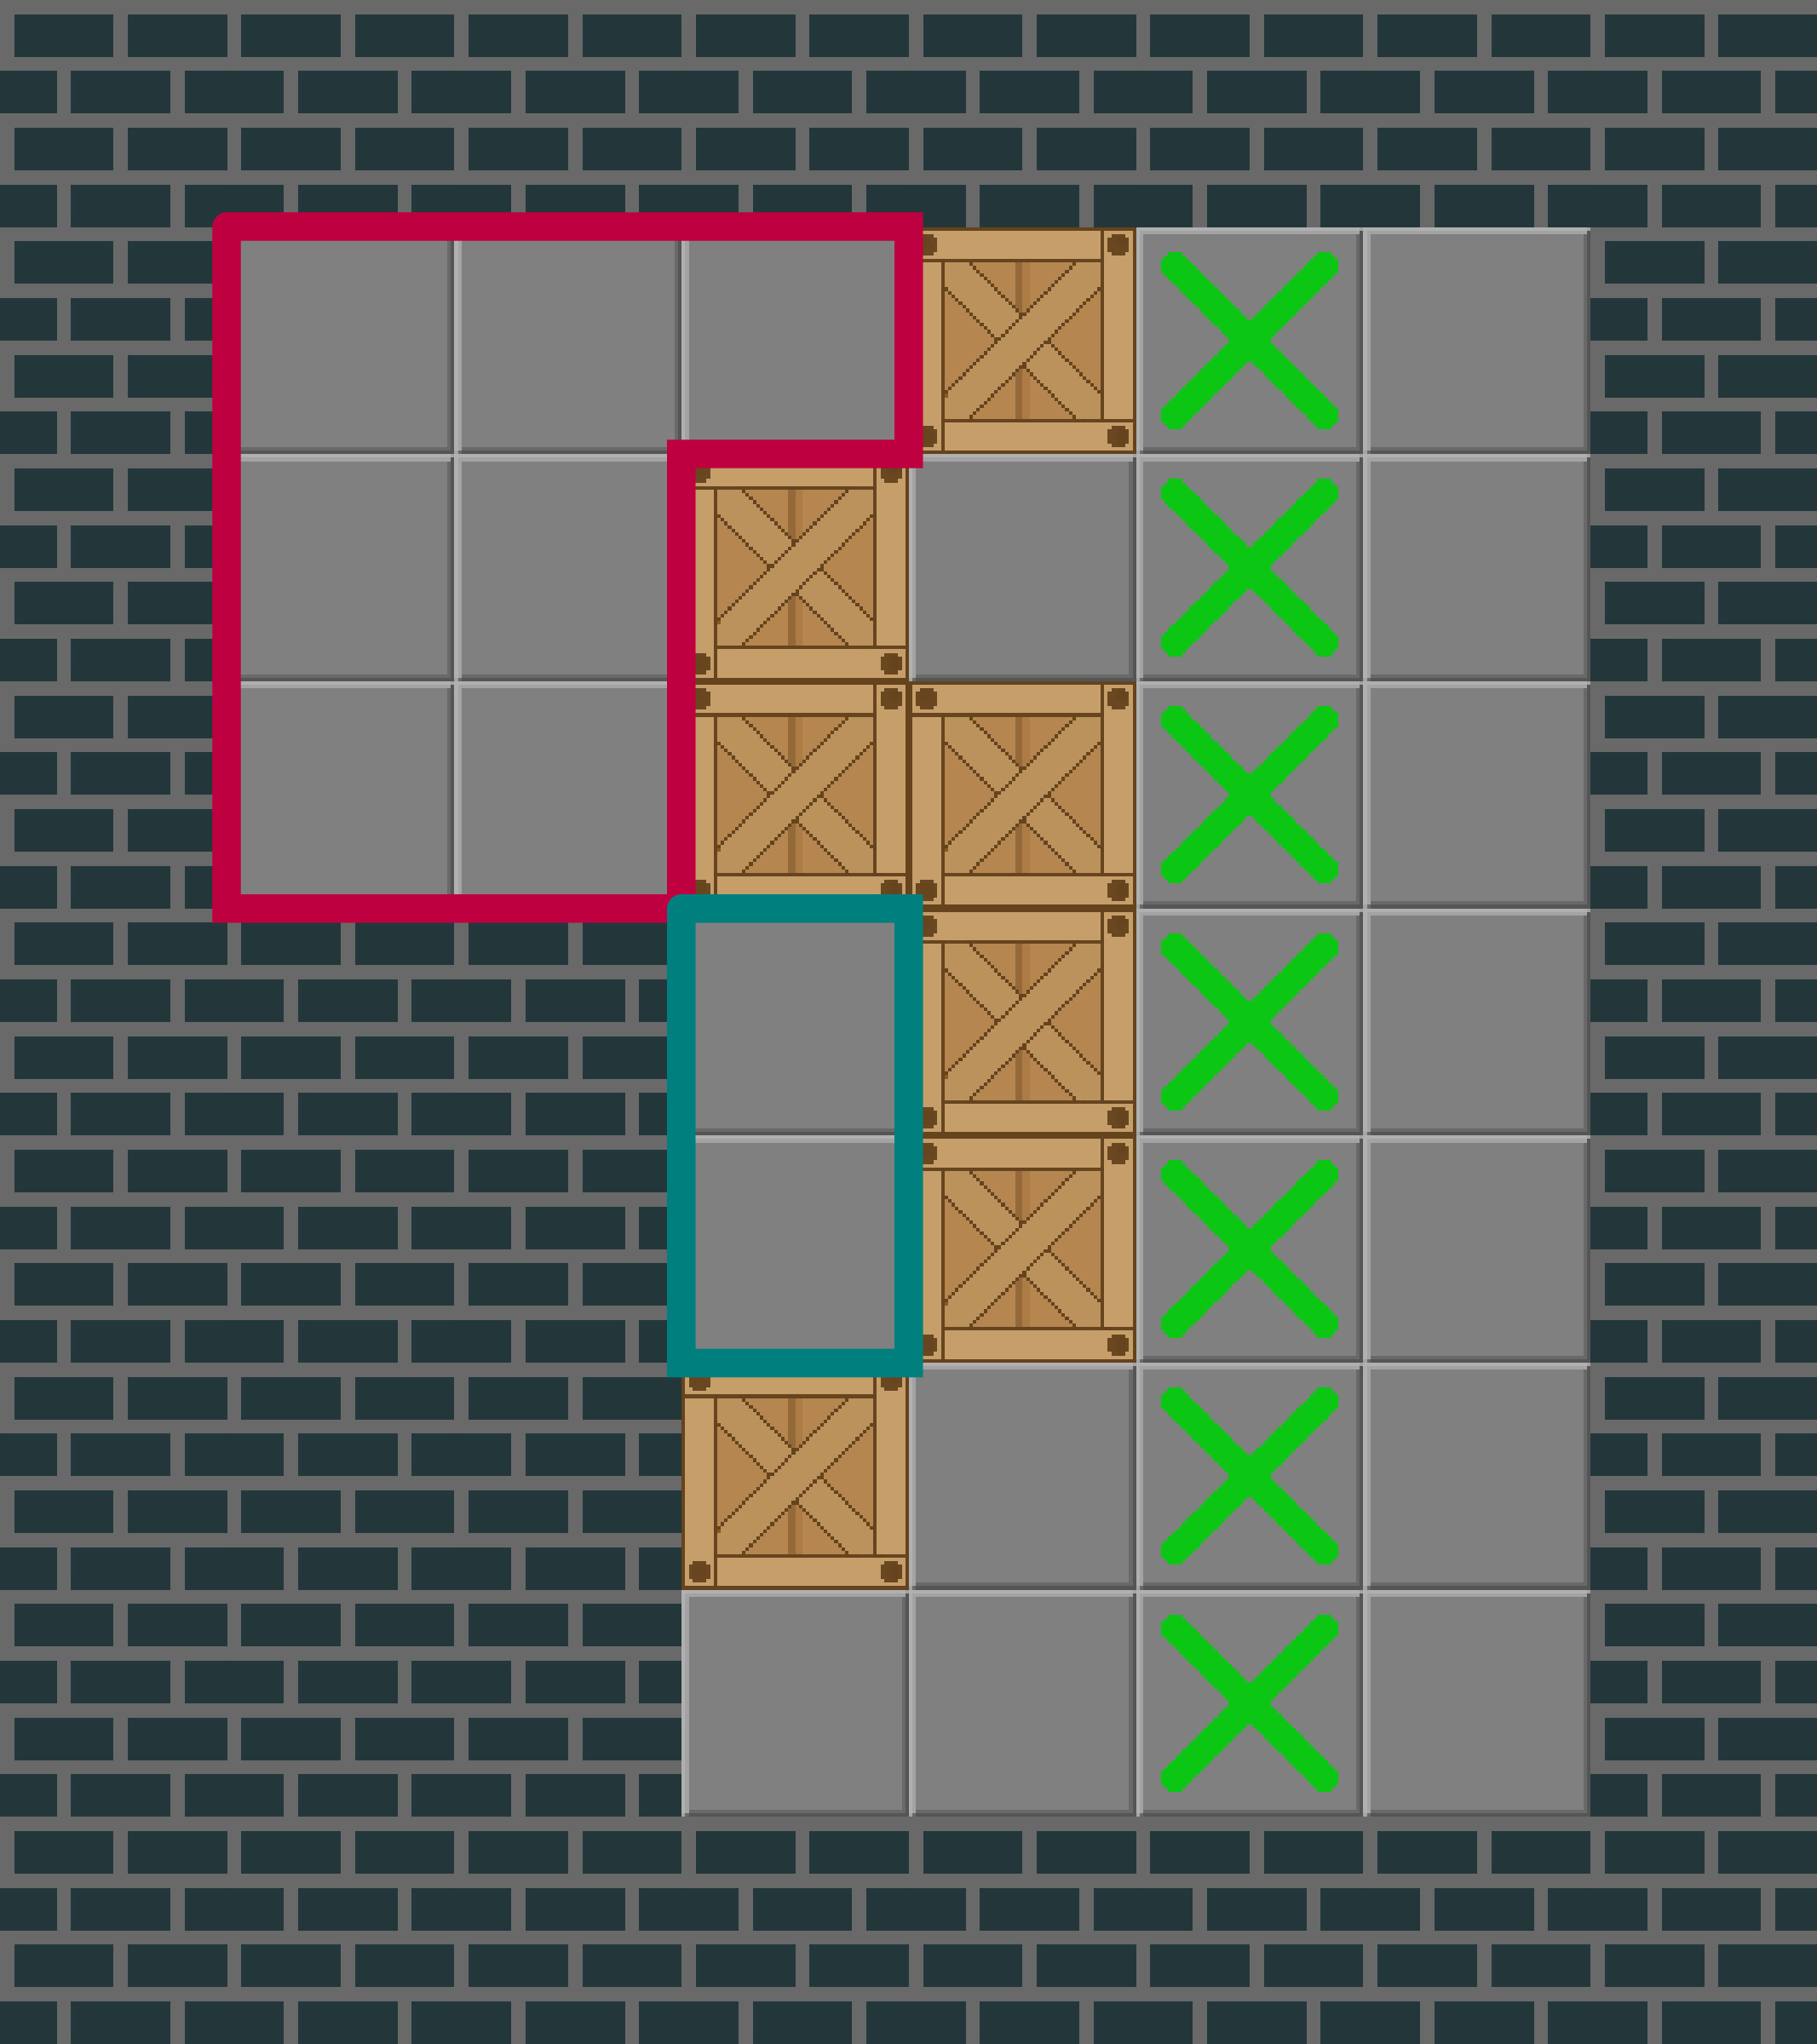
\includegraphics[width=\textwidth]{corral/multi_pi_corral_1.png}%

                        \centering
                        Deux \textit{I-Corrals}
                    \end{minipage}
                    \hfill
                    \begin{minipage}{0.45\textwidth}
                        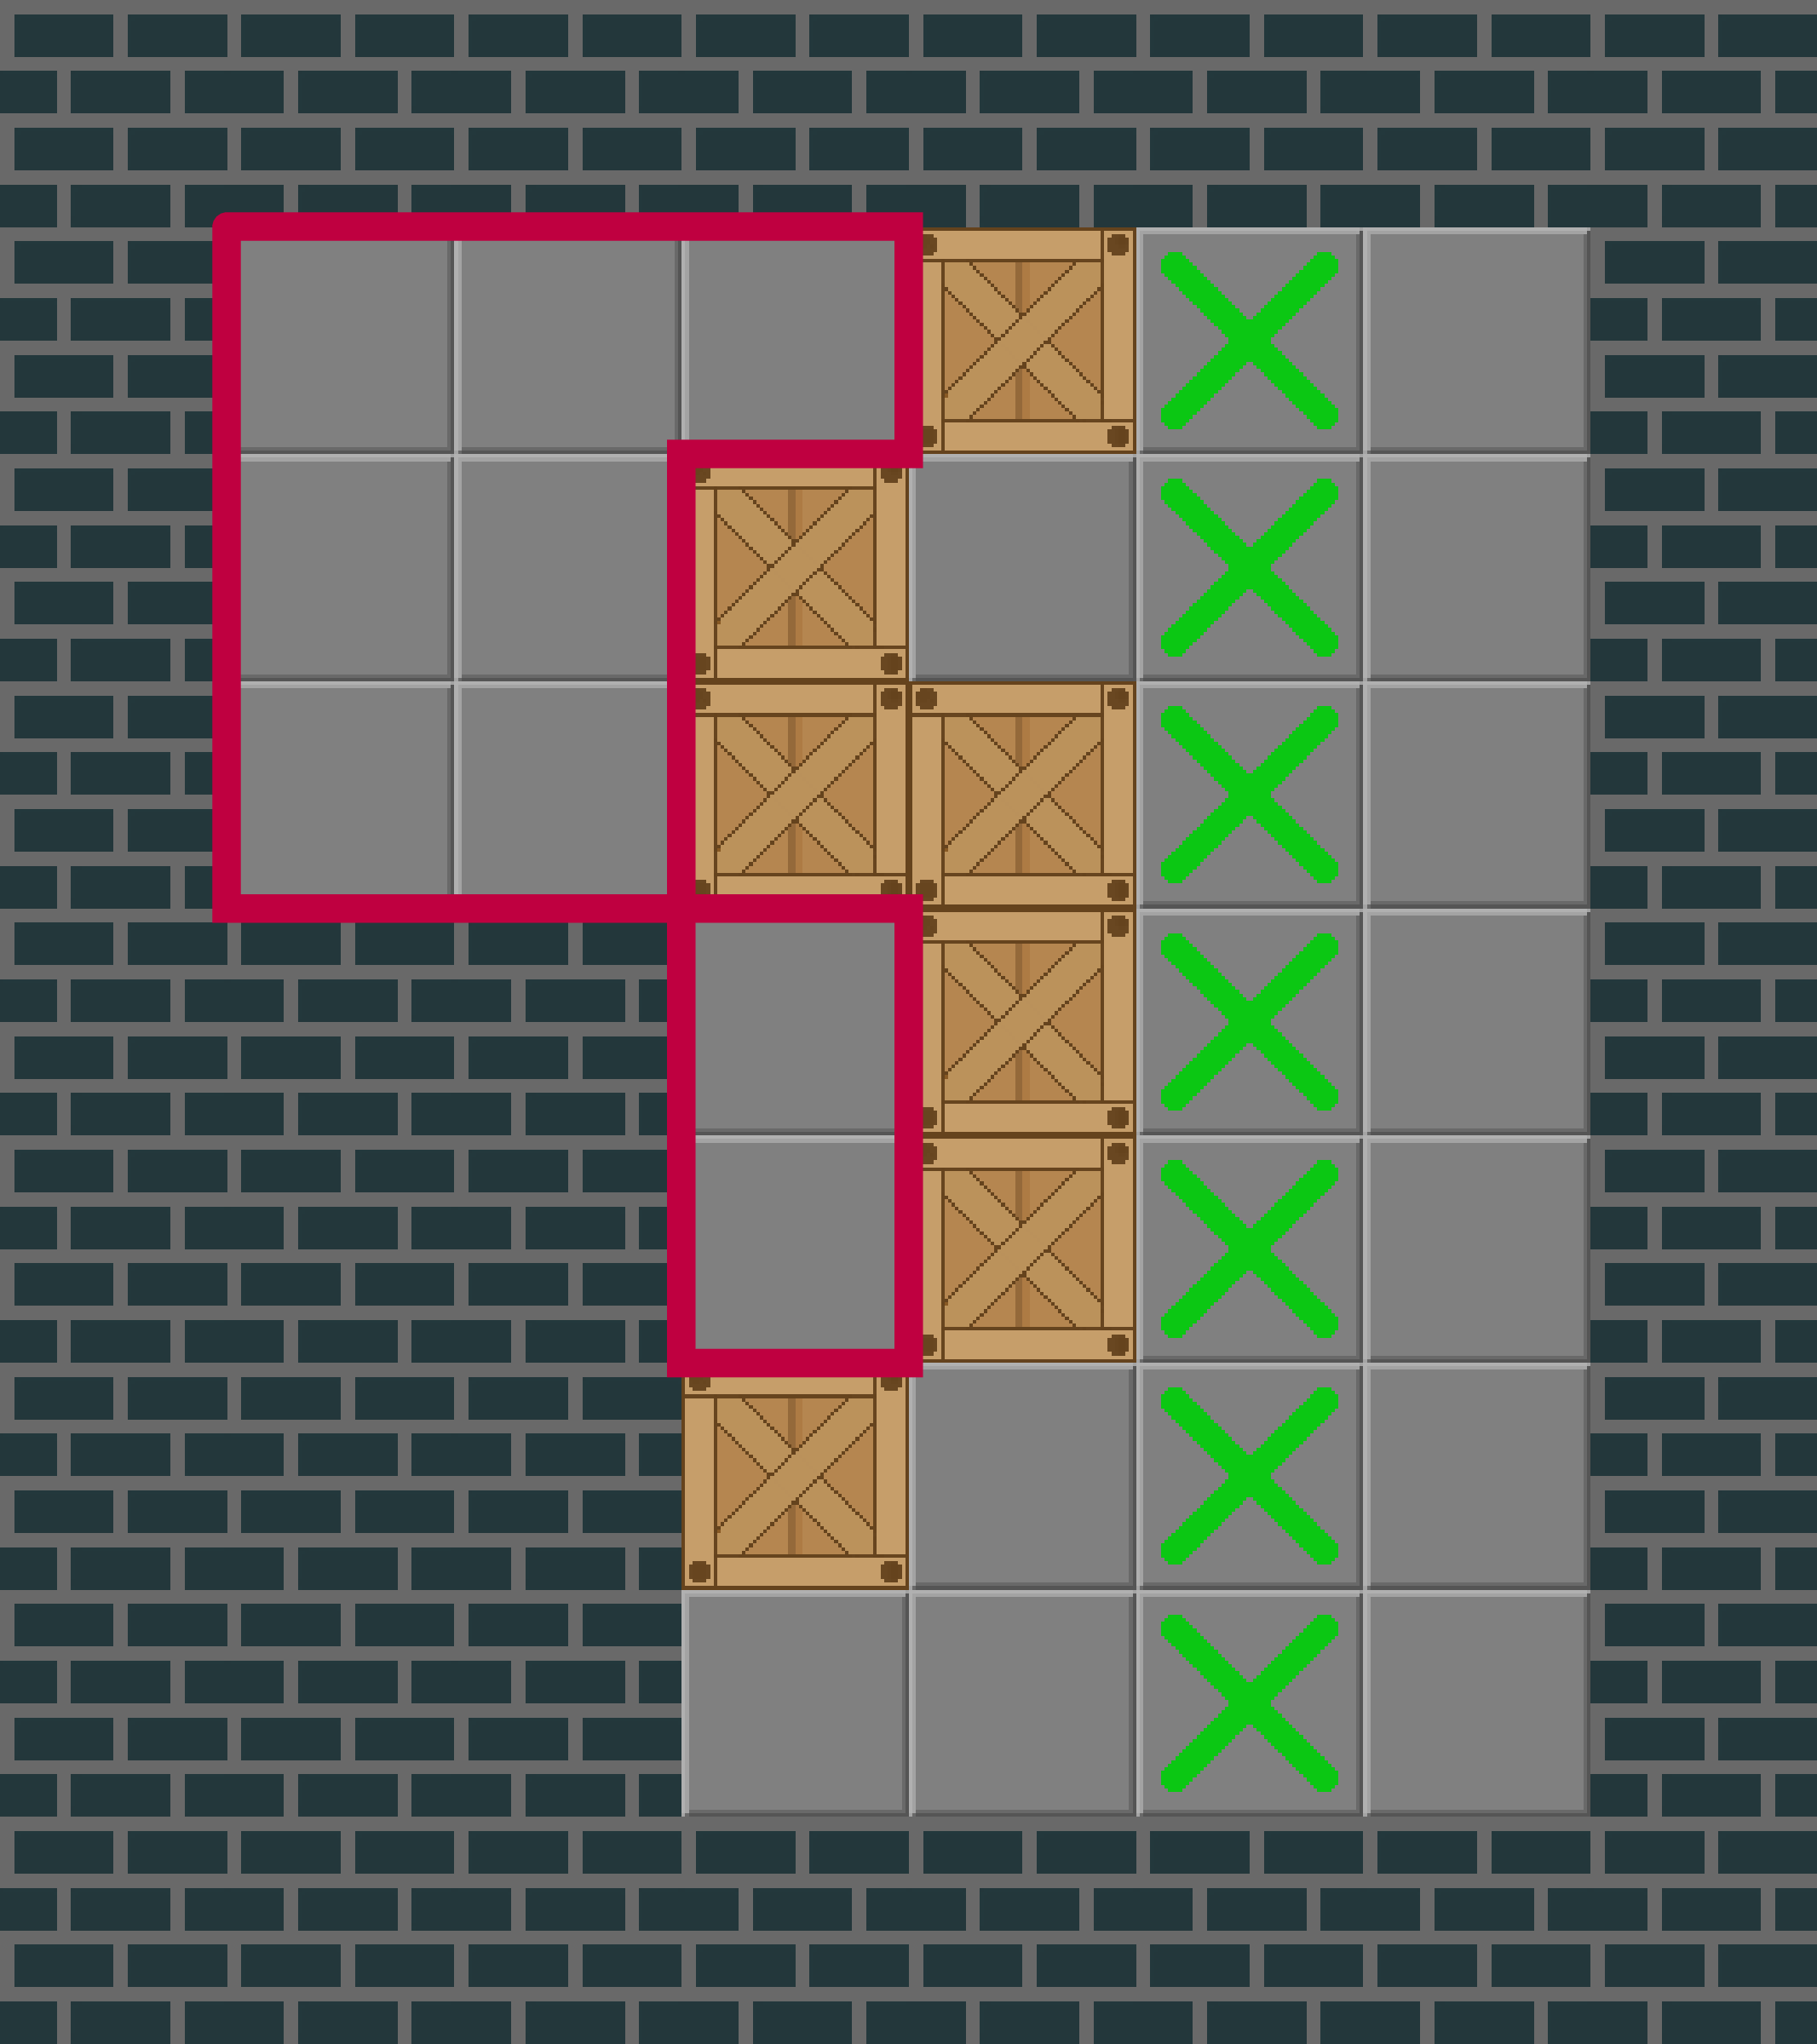
\includegraphics[width=\textwidth]{corral/multi_pi_corral_2.png}%

                        \centering
                        Un multi \textit{PI-Corral}
                    \end{minipage}
                }
                \only<3>{
                    \centering
                    Brian Damgaard: émonde l'arbre de recherche d'au moins \textbf{20\%} !
                }
            \end{frame}

            \begin{interstateframe}
                \begin{interstatenv}{6}{4}\interstatplot{5};\end{interstatenv}
            \end{interstateframe}

    \section{Recherche dirigée par une heuristique}
        \begin{frame}{Heuristique simple \textit{(Simple Lower Bound)}}
            \centering%
            \includegraphics[width=0.9\textwidth]{heuristics/simple.png}
            \Large$\boxed{2 + 4 + 3 = \mathbf{9}}$
        \end{frame}

        \begin{frame}{Heuristique gloutonne \textit{(Greedy Lower Bound)}}
            \centering
            \includegraphics[width=0.3\textwidth]{heuristics/greedy.png}

            \vspace{0.19cm}
            \begin{columns}
                \begin{column}{0.5\textwidth}
                    \begin{center}
                        \includegraphics[width=\textwidth]{heuristics/greedy_end.png}
                        \Large$\boxed{2 + 3 + 5 = \mathbf{10}}$
                    \end{center}
                \end{column}%

                \begin{column}{0.5\textwidth}
                    % Sorted table
                    \resizebox{0.9\textwidth}{!}{
                        \begin{tabular}{ | c | c | }
                            \hline
                                Caisse $\rightarrow$ Cible & Distance \\
                            \hline
                            $\mathbf{1 \rightarrow B}$ & \textbf{2} \\
                            \hline
                            $1 \rightarrow A$ & 3 \\
                            \hline
                            $1 \rightarrow C$ & 3 \\
                            \hline
                            $\mathbf{3 \rightarrow C}$ & \textbf{3} \\
                            \hline
                            $2 \rightarrow B$ & 4 \\
                            \hline
                            $3 \rightarrow B$ & 4 \\
                            \hline
                            $2 \rightarrow A$ & 5 \\
                            \hline
                            $2 \rightarrow C$ & 5 \\
                            \hline
                            $\mathbf{3 \rightarrow A}$ & \textbf{5} \\
                            \hline
                        \end{tabular}
                    }
                \end{column}
            \end{columns}
        \end{frame}

        \begin{interstateframe}
            \begin{interstatenv}{11}{5}\interstatplot{6};\end{interstatenv}
        \end{interstateframe}

        \begin{frame}{Vers FESS}
            \begin{itemize}
                \item FESS: algorithme utilisé par Festival, meilleur solveur.
                \item Ordre de priorité:
                    \begin{itemize}
                        \item maximiser le nombre de caisses rangées.
                        \item minimiser le nombre de \textit{corral}.
                        \item minimiser l'heuristique précédente.
                    \end{itemize}
            \end{itemize}
        \end{frame}

        \begin{interstateframe}
            \begin{interstatenv}{15}{4}\interstatplot{7};\end{interstatenv}
        \end{interstateframe}

    \section{Résultats}
        \begin{frame}{Nombre de niveaux résolus}
            \centering
            Limite de temps: 10 min. Limite de RAM: 32 Gio.

            \vspace{0.42cm}
            \begin{tabular}{|c|c|c|}
                \hline
                Ensemble de niveaux            & XSokoban    & \textit{Large test suite} \\
                \hline
                Nombre de niveaux              & 90          & 3272 \\
                \hline
                \textbf{A*}                    & \textbf{11} & \textbf{2204} \\
                \hline
                \textbf{fess0}                 & \textbf{15} & \textbf{2273} \\
                \hline
                Festival (Yaron Shoham)        & 90          & 3202 \\
                \hline
                Sokolution (Florent Diedler)   & 90          & 3130 \\
                \hline
                Takaken (Ken'ichiro Takahashi) & 90          & 2944 \\
                \hline
                YASS (Brian Damgaard)          & 89          & 2865 \\
                \hline
            \end{tabular}

            \BottomLeftText{Statistiques (pour les autres solveurs) par Matthias Meger et Brian Damgaard
                            (\href{https://sourceforge.net/projects/sokoban-solver-statistics/}{https://sourceforge.net/projects/sokoban-solver-statistics/})}
        \end{frame}

        \begin{frame}{Statistiques}
            \centering

            Temps moyen passé par niveaux

            \vspace{0.05cm}
            \resizebox{\textwidth}{!}{
                \begin{tabular}{|c|c|c|c|c|c|c|}
                    \hline
                    Solveur     & \textbf{A*}       & \textbf{fess0}    & Festival & Sokolution & Takaken & YASS \\
                    \hline
                    Temps moyen & \textbf{3min 28s} & \textbf{3min 16s} & 3s & 2s & 7s & 24s \\
                    \hline
                \end{tabular}
            }

            \vspace{0.3cm}
            Nombre de niveaux résolus (cumulés) en fonction du temps

            \resizebox{0.75\textwidth}{!}{
                \begin{tikzpicture}
                    \begin{axis}[
                            grid=major,
                            xmin=1, xmax=10,
                            ymin=2000, ymax=3300,
                            xlabel = {Temps (minutes)},
                            ylabel = {Nombre de niveaux},
                            legend entries={sokoshell, Festival, Sokolution, Takaken, YASS},
                            legend style={at={(1.5, 0.5)},anchor= east},
                            cycle list name=mylist
                        ]

                        \addplot table[x=min, y=sokoshell] {content/number_solved_per_minutes_data.txt};
                        \addplot table[x=min, y=Festival] {content/number_solved_per_minutes_data.txt};
                        \addplot table[x=min, y=Sokolution] {content/number_solved_per_minutes_data.txt};
                        \addplot table[x=min, y=Takaken] {content/number_solved_per_minutes_data.txt};
                        \addplot table[x=min, y=YASS] {content/number_solved_per_minutes_data.txt};
                    \end{axis}
                \end{tikzpicture}

            }

            \BottomLeftText{Statistiques (pour les autres solveurs) par Matthias Meger et Brian Damgaard
                            (\href{https://sourceforge.net/projects/sokoban-solver-statistics/}{https://sourceforge.net/projects/sokoban-solver-statistics/})}
        \end{frame}

        \begin{frame}[fragile]{Statistiques}
            \centering

            Pourcentage de niveaux résolus selon la composition des niveaux

            \vspace{0.42cm}
            \resizebox{0.9\textwidth}{!}{
                \begin{tikzpicture}
                    \begin{axis}[
                            name=ax1,
                            grid=major,
                            xmin=0, xmax=250,
                            ymin=0, ymax=100,
                            xlabel = {Nombre de sols},
                            % ylabel = {Pourcentage de niveaux résolus},
                            xlabel style = {yshift=-0.2cm, font=\LARGE},
                            cycle list name=mylist
                        ]
                        \addplot table[x=floors, y=sokoshell]
                            {content/Solved_levels_versus_floors__percent.txt};
                        \addplot table[x=floors, y=Festival]
                            {content/Solved_levels_versus_floors__percent.txt};
                        \addplot table[x=floors, y=Sokolution]
                            {content/Solved_levels_versus_floors__percent.txt};
                        \addplot table[x=floors, y=Takaken]
                            {content/Solved_levels_versus_floors__percent.txt};
                        \addplot table[x=floors, y=YASS]
                            {content/Solved_levels_versus_floors__percent.txt};

                        % \legend{}
                    \end{axis}
                    \begin{axis}[
                            at={(ax1.south east)},
                            xshift=1cm,
                            grid=major,
                            xmin=0, xmax=75,
                            ymin=0, ymax=100,
                            yticklabels=\empty,
                            xlabel = {Nombre de caisses},
                            xlabel style = {yshift=-0.2cm, font=\LARGE},
                            legend columns=5,
                            legend entries={sokoshell, Festival, Sokolution, Takaken, YASS},
                            legend style={font=\Large, at={(-0.1, 1.1)}, anchor=south},
                            cycle list name=mylist
                        ]
                        \addplot table[x=crates, y=sokoshell]
                            {content/Solved_levels_versus_crates__percent.txt};
                        \addplot table[x=crates, y=Festival]
                            {content/Solved_levels_versus_crates__percent.txt};
                        \addplot table[x=crates, y=Sokolution]
                            {content/Solved_levels_versus_crates__percent.txt};
                        \addplot table[x=crates, y=Takaken]
                            {content/Solved_levels_versus_crates__percent.txt};
                        \addplot table[x=crates, y=YASS]
                            {content/Solved_levels_versus_crates__percent.txt};
                    \end{axis}
                \end{tikzpicture}
            }
            \BottomLeftText{Statistiques (pour les autres solveurs) par Matthias Meger et Brian Damgaard
                            (\href{https://sourceforge.net/projects/sokoban-solver-statistics/}{https://sourceforge.net/projects/sokoban-solver-statistics/})}
        \end{frame}

%    \section{Annexe}
%        \begin{frame}{Tableau des complexités - Statique}
%            $c$ nombre de caisses, $C$ nombre de cibles, $w$ longueur et $h$ largeur du niveau, $t$ nombre de tunnels, $r$ nombre de salles, $N$ nombre d'états dans la liste des états à explorer.
%
%            \only<1>{
%                \begin{tabular}{|p{0.45\textwidth}|p{0.45\textwidth}|}
%                    \hline
%                    \multicolumn{2}{|c|}{Statique} \\
%                    \hline
%                    \textit{Dead tiles}                    & $\mathcal{O}((wh)^2)$            \\
%                    Détection des tunnels                  & $\mathcal{O}((wh)^2)$            \\
%                    Propriété \textit{oneway} des tunnels  & $\mathcal{O}(twh)$               \\
%                    Détection des salles                   & $\mathcal{O}((wh)^2)$            \\
%                    \textit{Packing order}                 & $\mathcal{O}(rcwh)$              \\
%                    Précalcul des distances cibles-caisses & $\mathcal{O}(wh(Cwh + C\log C))$ \\
%                    \hline
%                \end{tabular}
%            }
%
%            \frametitle<2>{Tableau des complexités - Dynamique}
%            \only<2>{
%                \begin{tabular}{|p{0.45\textwidth}|p{0.45\textwidth}|}
%                    \hline
%                    \multicolumn{2}{|c|}{Dynamique} \\
%                    \hline
%                    \textit{Freeze deadlocks}       & $\mathcal{O}(c)$                   \\
%                    Détection des \textit{corrals}  & $\mathcal{O}(wh)$                  \\
%                    PI-\textit{corral deadlocks}    & Exponentielle                      \\
%                    Table de \textit{deadlocks}     & $\mathcal{O}(1)$                   \\
%                    Recherche des états enfants     & $\mathcal{O}(crwh)$                \\
%                    Ajout des états enfants (A*)    & $\mathcal{O}((wh)^2 + \log N)$     \\
%                    Ajout des états enfants (fess0) & $\mathcal{O}(c + (wh)^2 + \log N)$ \\
%                    \hline
%                \end{tabular}
%            }
%        \end{frame}
%
%         \begin{frame}{Table de \textit{deadlocks}}
%            \only<1>{
%                \begin{minipage}{0.45\textwidth}
%                    \includegraphics[width=\textwidth]{deadlock_table/init.png}%
%                \end{minipage}
%                \hfill
%                \begin{minipage}{0.45\textwidth}
%                    \includegraphics[width=\textwidth]{deadlock_table/new_deadlock.png}%
%                \end{minipage}
%            }
%            \only<2>{
%                \centering
\begin{tikzpicture}[grow=right, level distance=3cm, sibling distance=2.5cm]
    \node {\includegraphics[width=0.2\textwidth]{deadlock_table/init.png}}
        child {
            node {\includegraphics[width=0.2\textwidth]{deadlock_table/floor.png}}
            child {node {...}}
        }
        child {
            node {\includegraphics[width=0.2\textwidth]{deadlock_table/crate.png}}
            child [dashed] { node{\includegraphics[width=0.2\textwidth]{deadlock_table/leaf.png}}}
        }
        child {
            node {\includegraphics[width=0.2\textwidth]{deadlock_table/wall.png}}
            child {node {...}}
        };
\end{tikzpicture}
%            }
%        \end{frame}
%
%        \begin{frame}{Précalcul des distances caisses-cibles}
%            \centering
%            \begin{columns}[onlytextwidth]
%                \only<1>{
%                    \begin{column}{0.3\textwidth}
%                        \begin{tabular}{|c|c|c|c|}
%                            \hline
%                            \multirow{2}{2em}{Case} & \multicolumn{3}{|c|}{Distances} \\ \cline{2-4}
%                            & A & B & C \\ \hline
%                            0 & 1 & 3 & 3 \\ \hline
%                            1 & 2 & 2 & 2 \\ \hline
%                            2 & 3 & 1 & 3 \\ \hline
%                            3 & 0 & 2 & 2 \\ \hline
%                            4 & 1 & 1 & 1 \\ \hline
%                            5 & 2 & 0 & 2 \\ \hline
%                            6 & 1 & 3 & 1 \\ \hline
%                            7 & 2 & 2 & 0 \\ \hline
%                            8 & 3 & 1 & 1 \\ \hline
%                        \end{tabular}
%                    \end{column}
%                }%
%                \only<2>{
%                    \begin{column}{0.49\textwidth}
%                        \begin{tabular}{|c|c|c|c|}
%                            \hline
%                            \multirow{2}{2em}{Case} & \multicolumn{3}{|c|}{Distances} \\
%                            & \multicolumn{3}{|c|}{triées} \\ \hline
%                            0 & A: 1 & B: 3 & C: 3 \\ \hline
%                            1 & A: 2 & B: 2 & C: 2 \\ \hline
%                            2 & B: 1 & A: 3 & C: 3 \\ \hline
%                            3 & A: 0 & B: 2 & C: 2 \\ \hline
%                            4 & A: 1 & B: 1 & C: 1 \\ \hline
%                            5 & B: 0 & A: 2 & C: 2 \\ \hline
%                            6 & A: 1 & C: 1 & B: 3 \\ \hline
%                            7 & C: 0 & A: 2 & B: 2 \\ \hline
%                            8 & B: 1 & C: 1 & A: 3 \\ \hline
%                        \end{tabular}
%                    \end{column}
%                }
%                \begin{column}{0.5\textwidth}
%                    \includegraphics[width=\textwidth]{optimisations/distances.png}
%                \end{column}
%
%            \end{columns}
%        \end{frame}
%
%        \begin{frame}{\textit{Greedy Lower Bound} en $\mathcal{O}(n^2)$}
    \begin{minipage}{0.5\textwidth}
        % number from Aymeric_Du_Peloux_282 lvl4
        \centering
        \begin{tikzpicture}[list/.style={rectangle split, rectangle split parts=2,draw},
                            mat/.style={ampersand replacement=\&, nodes={draw, inner sep=.3333em}, inner sep=0}]
            { [start chain=going below]
                \only<1-2>{
                    \node [list, on chain] (A) {1};
                    \node [list, on chain] (B) {2};
                    \node [list, on chain] (C) {3};
                    \node [list, on chain] (D) {4};

                    \matrix [mat, right=of A] (a) {
                        \node (a11) {3}; \& \node (a12) {4}; \& \node (a13) {1}; \& \node (a14) {2}; \\ % target
                        \node (a21) {1}; \& \node (a22) {1}; \& \node (a23) {2}; \& \node (a24) {4}; \\ % distance
                    };

                    \matrix [mat, right=of B] (b) {
                        \node (b11) {1}; \& \node (b12) {3}; \& \node (b13) {4}; \& \node (b14) {2}; \\
                        \node (b21) {1}; \& \node (b22) {2}; \& \node (b23) {2}; \& \node (b24) {3}; \\
                    };

                    \matrix [mat, right=of C] (c) {
                        \node (c11) {1}; \& \node (c12) {4}; \& \node (c13) {2}; \& \node (c14) {3}; \\
                        \node (c21) {2}; \& \node (c22) {3}; \& \node (c23) {4}; \& \node (c24) {5}; \\
                    };

                    \matrix [mat, right=of D] (d) {
                        \node (d11) {1}; \& \node (d12) {3}; \& \node (d13) {4}; \& \node (d14) {2}; \\
                        \node (d21) {3}; \& \node (d22) {4}; \& \node (d23) {4}; \& \node (d24) {5}; \\
                    };

                    \draw [*->] (A.two) -- (B);
                    \draw [*->] (B.two) -- (C);
                    \draw [*->] (C.two) -- (D);

                    \draw [*->] (A.two) -- (a);
                    \draw [*->] (B.two) -- (b);
                    \draw [*->] (C.two) -- (c);
                    \draw [*->] (D.two) -- (d);

                    \draw [->] ($(a11)+(0,0.7cm)$) -- (a11);
                    \draw [->] ($(b11)+(0,0.7cm)$) -- (b11);
                    \draw [->] ($(c11)+(0,0.7cm)$) -- (c11);
                    \draw [->] ($(d11)+(0,0.7cm)$) -- (d11);
                }

                \only<2>{
                    \node [draw, ellipse, red] at (b21) {};

                    \draw (a13.north west) -- (a23.south east);
                    \draw (a13.north east) -- (a23.south west);

                    \draw (c11.north west) -- (c21.south east);
                    \draw (c11.north east) -- (c21.south west);

                    \draw (d11.north west) -- (d21.south east);
                    \draw (d11.north east) -- (d21.south west);
                }

                \only<3-4>{
                    \node [list, on chain] (A) {1};
                    \node [list, on chain] (C) {3};
                    \node [list, on chain] (D) {4};

                    \matrix [mat, right=of A] (a) {
                        \node (a11) {3}; \& \node (a12) {4}; \& \node (a13) {1}; \& \node (a14) {2}; \\ % target
                        \node (a21) {1}; \& \node (a22) {1}; \& \node (a23) {2}; \& \node (a24) {4}; \\ % distance
                    };

                    \matrix [mat, right=of C] (c) {
                        \node (c11) {1}; \& \node (c12) {4}; \& \node (c13) {2}; \& \node (c14) {3}; \\
                        \node (c21) {2}; \& \node (c22) {3}; \& \node (c23) {4}; \& \node (c24) {5}; \\
                    };

                    \matrix [mat, right=of D] (d) {
                        \node (d11) {1}; \& \node (d12) {3}; \& \node (d13) {4}; \& \node (d14) {2}; \\
                        \node (d21) {3}; \& \node (d22) {4}; \& \node (d23) {4}; \& \node (d24) {5}; \\
                    };

                    \draw [*->] (A.two) -- (C);
                    \draw [*->] (C.two) -- (D);

                    \draw [*->] (A.two) -- (a);
                    \draw [*->] (C.two) -- (c);
                    \draw [*->] (D.two) -- (d);


                    \draw (a13.north west) -- (a23.south east);
                    \draw (a13.north east) -- (a23.south west);

                    \draw (c11.north west) -- (c21.south east);
                    \draw (c11.north east) -- (c21.south west);

                    \draw (d11.north west) -- (d21.south east);
                    \draw (d11.north east) -- (d21.south west);
                }

                \only<3>{
                    \draw [->] ($(a11)+(0,0.7cm)$) -- (a11);
                    \draw [->] ($(c11)+(0,0.7cm)$) -- (c11);
                    \draw [->] ($(d11)+(0,0.7cm)$) -- (d11);
                }

                \only<4>{
                    \node [draw, ellipse, red] at (a21) {};

                    \draw (c14.north west) -- (c24.south east);
                    \draw (c14.north east) -- (c24.south west);

                    \draw (d12.north west) -- (d22.south east);
                    \draw (d12.north east) -- (d22.south west);

                    \draw [->] ($(a11)+(0,0.7cm)$) -- (a11);
                    \draw [->] ($(c12)+(0,0.7cm)$) -- (c12);
                    \draw [->] ($(d12)+(0,0.7cm)$) -- (d12);
                }

                \only<5-6>{
                    \node [list, on chain] (C) {3};
                    \node [list, on chain] (D) {4};

                    \matrix [mat, right=of C] (c) {
                        \node (c11) {1}; \& \node (c12) {4}; \& \node (c13) {2}; \& \node (c14) {3}; \\
                        \node (c21) {2}; \& \node (c22) {3}; \& \node (c23) {4}; \& \node (c24) {5}; \\
                    };

                    \matrix [mat, right=of D] (d) {
                        \node (d11) {1}; \& \node (d12) {3}; \& \node (d13) {4}; \& \node (d14) {2}; \\
                        \node (d21) {3}; \& \node (d22) {4}; \& \node (d23) {4}; \& \node (d24) {5}; \\
                    };

                    \draw [*->] (C.two) -- (D);

                    \draw [*->] (C.two) -- (c);
                    \draw [*->] (D.two) -- (d);


                    \draw (c11.north west) -- (c21.south east);
                    \draw (c11.north east) -- (c21.south west);
                    \draw (c14.north west) -- (c24.south east);
                    \draw (c14.north east) -- (c24.south west);

                    \draw (d11.north west) -- (d21.south east);
                    \draw (d11.north east) -- (d21.south west);
                    \draw (d12.north west) -- (d22.south east);
                    \draw (d12.north east) -- (d22.south west);
                }

                \only<5>{
                    \draw [->] ($(c12)+(0,0.7cm)$) -- (c12);
                    \draw [->] ($(d12)+(0,0.7cm)$) -- (d12);
                }

                \only<6>{
                    \node [draw, ellipse, red] at (c22) {};

                    \draw (d13.north west) -- (d23.south east);
                    \draw (d13.north east) -- (d23.south west);

                    \draw [->] ($(c12)+(0,0.7cm)$) -- (c12);
                    \draw [->] ($(d13)+(0,0.7cm)$) -- (d13);
                }

                \only<7>{
                    \node [list, on chain] (D) {4};

                    \matrix [mat, right=of D] (d) {
                        \node (d11) {1}; \& \node (d12) {3}; \& \node (d13) {4}; \& \node (d14) {2}; \\
                        \node (d21) {3}; \& \node (d22) {4}; \& \node (d23) {4}; \& \node (d24) {5}; \\
                    };

                    \draw [*->] (D.two) -- (d);
                    \draw [->] ($(d14)+(0,0.7cm)$) -- (d14);

                    \draw (d11.north west) -- (d21.south east);
                    \draw (d11.north east) -- (d21.south west);
                    \draw (d12.north west) -- (d22.south east);
                    \draw (d12.north east) -- (d22.south west);
                    \draw (d13.north west) -- (d23.south east);
                    \draw (d13.north east) -- (d23.south west);

                    \node [draw, ellipse, red] at (d24) {};
                }
            }
        \end{tikzpicture}
    \end{minipage}
    \begin{minipage}{0.4\textwidth}
        \begin{center}
            \only<1>{$h=$}
            \only<2-3>{$h=1+$}
            \only<4-5>{$h=1+1+$}
            \only<6>{$h=1+1+3+$}
            \only<7>{$h=1+1+3+5=10$}
        \end{center}
    \end{minipage}
\end{frame}
%
%        \begin{frame}{Parcours de graphes: démarquer tous les nœuds en $\mathcal{O}(1)$}
%
%            \centering
%            nœud marqué \textit{ssi valeur} $= m$
%
%            \begin{tikzpicture}
%                \node (start) {
%                    \includegraphics[width=0.15\textwidth]{optimisations/mark_init.png}
%                };
%                \node[right=of start] (first) {
%                    \includegraphics[width=0.15\textwidth]{optimisations/mark_player.png}
%                };
%                \node[right=of first] (second) {
%                    \includegraphics[width=0.15\textwidth]{optimisations/mark_all.png}
%                };
%                \node[right=of second] (third) {
%                    \includegraphics[width=0.15\textwidth]{optimisations/unmark.png}
%                };
%                % don't remove '0cm', otherwise tikz will place the text too below
%                \node [above=0cm of start.north] {$m=0$};
%                \node [above=0cm of first.north] {$m=0$};
%                \node [above=0cm of second.north] {$m=0$};
%                \node [above=0cm of third.north] {$m=1$};
%
%                \draw[->, line width=\arrowwidth] (start.east)  -- (first.west);
%                \draw[->, line width=\arrowwidth, dashed] (first.east) -- (second.west);
%                \draw[->, line width=\arrowwidth] (second.east) -- (third.west);
%            \end{tikzpicture}
%        \end{frame}
%
%        \begin{frame}{Calcul des \textit{corrals} en $\mathcal{O}(wh)$}
%            \only<1>{
%                Utilisation de \textit{Union-Find}: partition de $\llbracket 0;wh-1 \rrbracket$.
%
%                \vspace{0.1cm}
%                \begin{columns}
%                    \begin{column}{0.4\textwidth}
%                        \centering
%                        \includegraphics[width=\textwidth]{corral_detection/corral.png}
%                    \end{column}
%                    \begin{column}{0.4\textwidth}
%                        \centering
%                        \includegraphics[width=\textwidth]{corral_detection/corral_union_find.png}
%                    \end{column}
%                \end{columns}
%            }
%            \only<2-10>{
%                \centering
%                \begin{tikzpicture}[remember picture]
%                    \node[visible on=<2-5>] (A) {
%                        \includegraphics[width=0.32\textwidth]{corral_detection/corral_start.png}
%                    };
%                    \node[visible on=<3-5>, right=of A] (B) {
%                        \includegraphics[width=0.32\textwidth]{corral_detection/corral_1.png}
%                    };
%                    \node[visible on=<4-5>,below=of A] (C) {
%                        \includegraphics[width=0.32\textwidth]{corral_detection/corral_2.png}
%                    };
%                    \node[visible on=<5>, below=of B] (D) {
%                        \includegraphics[width=0.32\textwidth]{corral_detection/corral_3.png}
%                    };
%
%                    \draw[visible on=<3-5>, ->, line width=\arrowwidth] (A.east) -- (B.west);
%
%                    \coordinate (I) at ($ (B) ! .5 ! (C) $);
%                    \draw[visible on=<4-5>, ->, line width=\arrowwidth] (B.south) |- (I) -| (C.north);
%                    \draw[visible on=<5>, ->, line width=\arrowwidth, dashed] (C.east) -- (D.west);
%
%
%
%                    \node[visible on=<6-9>] (A) {%
%                        \includegraphics[width=0.32\textwidth]{corral_detection/corral_4.png}%
%                    };%
%                    \node[visible on=<7-9>, right=of A] (B) {%
%                        \includegraphics[width=0.32\textwidth]{corral_detection/corral_5.png}%
%                    };%
%                    \node[visible on=<8-9>,below=of A] (C) {%
%                        \includegraphics[width=0.32\textwidth]{corral_detection/corral_6.png}%
%                    };%
%                    \node[visible on=<9>, below=of B] (D) {%
%                        \includegraphics[width=0.32\textwidth]{corral_detection/corral_7.png}%
%                    };%
%
%                    \draw[visible on=<7-9>, ->, line width=\arrowwidth, dashed] (A.east) -- (B.west);
%
%                    \coordinate (I) at ($ (B) ! .5 ! (C) $);
%                    \draw[visible on=<8-9>, ->, line width=\arrowwidth] (B.south) |- (I) -| (C.north);
%                    \draw[visible on=<9>, ->, line width=\arrowwidth] (C.east) -- (D.west);
%
%                    \node[visible on=<10>] (A) {%
%                        \includegraphics[width=0.32\textwidth]{corral_detection/corral_8.png}%
%                    };%
%                \end{tikzpicture}
%            }
%
%            \onslide<6> {
%                \begin{tikzpicture}[overlay, remember picture]
%                    \draw[->, line width=\arrowwidth]
%                    let \p1 = (current page.south west), \p2 = (A.west) in
%                    (\x1, \y2) -- (\p2);
%                \end{tikzpicture}
%            }
%            \onslide<10> {
%                \begin{tikzpicture}[overlay, remember picture]
%                    \draw[->, line width=\arrowwidth, dashed]
%                    let \p1 = (current page.south west), \p2 = (A.west) in
%                    (\x1, \y2) -- (\p2);
%                \end{tikzpicture}
%            }
%        \end{frame}
\end{document}
